\pdfoutput=1
\pdfcompresslevel=9
\pdfinfo
{
    /Author (Autor)
    /Title (Tytul)
    /Subject (Tematyka)
    /Keywords (Slowa kluczowe)
}
%\documentclass[a4paper,polish,onecolumn,oneside,floatssmall,11pt,titleauthor,wide,openright]{mwrep}
%\usepackage[scale={0.7,0.8},paper=a4paper,twoside]{geometry}
\documentclass[a4paper,onecolumn,oneside,11pt,wide,floatssmall]{mwrep}
% \usepackage{polish}
\usepackage{amsmath}
\usepackage{amsfonts}
\usepackage{amssymb}
\usepackage{amsthm}
\usepackage{bookman}
\usepackage{enumerate}
\usepackage{rotating}

\usepackage{geometry}
\usepackage[utf8]{inputenc}
\usepackage[T1]{fontenc}
% \usepackage{t1enc}
% \usepackage[pdftex, bookmarks]{hyperref}
\usepackage[pdftex, bookmarks=false]{hyperref}
\def\url#1{{ \tt #1}}

\usepackage{listings}

% marginesy
\textwidth\paperwidth
\advance\textwidth -55mm
\oddsidemargin-0.9in
\advance\oddsidemargin 33mm
\evensidemargin-0.9in
\advance\evensidemargin 33mm
\topmargin -1in
\advance\topmargin 25mm
\setlength\textheight{48\baselineskip}
\addtolength\textheight{\topskip}
\marginparwidth15mm

\clubpenalty=10000 % to kara za sierotki
\widowpenalty=10000 % nie pozostawia wdów
\brokenpenalty=10000 % nie dzieli wyrazów pomiędzy stronami
\sloppy

\tolerance4500
\pretolerance250
\hfuzz=1.5pt
\hbadness1450

% ŻYWA PAGINA
\renewcommand{\chaptermark}[1]{\markboth{\scshape\small\bfseries \
#1}{\small\bfseries \ #1}}
\renewcommand{\sectionmark}[1]{\markboth{\scshape\small\bfseries\thesection.\
#1}{\small\bfseries\thesection.\ #1}}
\newcommand{\headrulewidth}{0.5pt}
\newcommand{\footrulewidth}{0.pt}
\pagestyle{uheadings}

\usepackage[pdftex]{color,graphicx}
\usepackage[polish]{babel}

% \textheight232mm
% \setlength{\textwidth}{\textwidth}
% \setlength{\oddsidemargin}{\evensidemargin}
% \setlength{\evensidemargin}{0.3cm}
\usepackage[sort, compress]{cite}

%\usepackage{multibib}
%\newcites{bk,st,doc,web}{Książki i~artykuły,Standardy i~zalecenia,Dokumentacja produktów,Publikacje i~serwisy internetowe}

\theoremstyle{definition}
\newtheorem{defn}{Definicja}[section]
\newtheorem{conj}{Teza}[section]
\newtheorem{conjmain}{Teza}
\newtheorem{exmp}{Przykład}[section]

\theoremstyle{plain}% default
\newtheorem{thm}{Twierdzenie}[section]
\newtheorem{lem}[thm]{Lemat}
\newtheorem{prop}[thm]{Hipoteza}
\newtheorem*{cor}{Wniosek}

\theoremstyle{remark}
\newtheorem*{rem}{Uwaga}
\newtheorem*{note}{Uwaga}
\newtheorem{case}{Przypadek}

\definecolor{ListingBackground}{rgb}{0.95,0.95,0.95}

\begin{document}

% kody źródłowe wplatane w tekst
\lstdefinestyle{incode}
{
basicstyle={\footnotesize},
keywordstyle={\bf\footnotesize\color{blue}},
commentstyle={\em\footnotesize\color{magenta}},
numbers=left,
stepnumber=5,
firstnumber=1,
numberfirstline=true,
numberblanklines=true,
numberstyle={\sf\tiny},
numbersep=10pt,
tabsize=2,
xleftmargin=17pt,
framexleftmargin=3pt,
framexbottommargin=2pt,
framextopmargin=2pt,
framexrightmargin=0pt,
showstringspaces=true,
backgroundcolor={\color{ListingBackground}},
extendedchars=true,
% title=\lstname,
captionpos=b,
% abovecaptionskip=1pt,
% belowcaptionskip=1pt,
frame=tb,
framerule=0pt,
}

% kody źródłowe z podpisem
\lstdefinestyle{outcode}
{
basicstyle={\footnotesize},
keywordstyle={\bf\footnotesize\color{blue}},
commentstyle={\em\footnotesize\color{magenta}},
numbers=left,
stepnumber=5,
firstnumber=1,
numberfirstline=true,
numberblanklines=true,
numberstyle={\sf\tiny},
numbersep=10pt,
tabsize=2,
xleftmargin=17pt,
framexleftmargin=3pt,
framexbottommargin=2pt,
framextopmargin=2pt,
framexrightmargin=0pt,
showstringspaces=true,
backgroundcolor={\color{ListingBackground}},
extendedchars=true,
% title=\lstname,
captionpos=b,
% abovecaptionskip=1pt,
% belowcaptionskip=1pt,
frame=tb,
framerule=0.1pt,
}

\renewcommand*\lstlistingname{Wydruk}
\renewcommand*\lstlistlistingname{Spis wydruków}

\pagenumbering{roman}
\renewcommand{\baselinestretch}{1.0}
\raggedbottom

\begin{titlepage}
    % Strona tytułowa
    \vbox to\textheight{\hyphenpenalty=10000
    \begin{center}
	\begin{tabular}{p{107mm} p{9cm}}
	    \begin{minipage}{9cm}
	      \begin{center}
	      Politechnika Warszawska \\
	      Wydział Elektroniki i Technik Informacyjnych \\
	      Instytut Automatyki i Informatyki Stosowanej
	      \end{center}
	    \end{minipage}
	    &
	    \begin{minipage}{8cm}
	    \begin{flushleft}
	     \footnotesize
	      Rok akademicki 2012/2013
	    \vspace*{2.75\baselineskip}
	    \end{flushleft}
	    \end{minipage} \\
	\end{tabular}
	\vspace*{3.75\baselineskip}
	\par\vspace{\smallskipamount}
	\vspace*{2\baselineskip}{\LARGE Praca dyplomowa inżynierska\par}
	\vspace{3\baselineskip}{\LARGE\strut Cezary Guz\par}
	\vspace*{2\baselineskip}{\huge\bfseries Odległość, podobieństwo i niepodobieństwo obrazów na przykładzie odcisków palców\par}

	\vspace*{7\baselineskip}
	\hfill\mbox{}\par\vspace*{\baselineskip}\noindent
	\begin{tabular}[b]{@{}p{3cm}@{\ }l@{}}
	    {\large\hfill } & {\large }
	\end{tabular}
	\hfill
	\begin{tabular}[b]{@{}l@{}}
	Opiekun pracy: \\[\smallskipamount]
	{\large prof. dr hab. Andrzej Pacut}
	\end{tabular}\par
	\vspace*{4\baselineskip}
    \begin{tabular}{p{\textwidth}}
    \begin{flushleft}
	\begin{minipage}{7cm}
	Ocena \dotfill
	\par\vspace{1.6\baselineskip}
	\dotfill
	\par\noindent
	\centerline{\footnotesize Podpis Przewodniczącego} \par
	\centerline{\footnotesize Komisji Egzaminu Dyplomowego}\par
	\end{minipage}
    \end{flushleft}
    \end{tabular}
    \end{center}}

    % Życiorys
    \newpage\thispagestyle{empty}
    \begin{tabular}{p{5cm} p{12cm}}
    \begin{minipage}{5cm}
    \center
    
\includegraphics[height=6.5cm,width=4.5cm]{img/foto.jpg}
    \end{minipage}
    &
    \begin{minipage}{12cm}
    \begin{flushleft}
    \par\noindent\vspace{1\baselineskip}
    \begin{tabular}[h]{l l}
    {\normalsize\it Specjalność:} & Informatyka -- \\
    & Systemy informacyjno decyzyjne
    \end{tabular}
    \par\noindent\vspace{1\baselineskip}
    \begin{tabular}[h]{l l}
    {\normalsize\it Data urodzenia:} & {\normalsize 8 stycznia 1989 r.}
    \end{tabular}
    \par\noindent\vspace{1\baselineskip}
    \begin{tabular}[h]{l l}
    {\normalsize\it Data rozpoczęcia studiów:} & {\normalsize 1 października 2008 r.}
    \end{tabular}
    \par\noindent\vspace{1\baselineskip}
    \end{flushleft}
    \end{minipage}
    \end{tabular}
    \vspace*{1\baselineskip}
    \begin{center}
	{\large\bfseries Życiorys}\par\bigskip
    \end{center}

    \indent
    Nazywam się  Guz Cezary urodziłem się 8 stycznia 1989r. w Lubartowie. W 2005 roku ukończyłem Publiczne gimnazjum Nr 4 im Komisji Edukacji Narodowej w Puławach. Swoją edukację następnie kontynuowałem w II liceum ogólnokształcącym im. Komisji Edukacji Narodowej w Puławach, w klasie o profilu matematyczno-fizyczno-informatycznym. W październiku 2008 roku rozpocząłem studia na wydziale Elektroniki i Technik Informacyjnych Politechniki Warszawskiej na kierunku Informatyka.
    \par
    \vspace{2\baselineskip}
    \hfill\parbox{15em}{{\small\dotfill}\\[-.3ex]
    \centerline{\footnotesize podpis studenta}}\par
    \vspace{3\baselineskip}
    \begin{center}
 	{\large\bfseries Egzamin dyplomowy} \par\bigskip\bigskip
    \end{center}
    \par\noindent\vspace{1.5\baselineskip}
    Złożył egzamin dyplomowy w dn. \dotfill
    \par\noindent\vspace{1.5\baselineskip}
    Z wynikiem \dotfill
    \par\noindent\vspace{1.5\baselineskip}
    Ogólny wynik studiów \dotfill
    \par\noindent\vspace{1.5\baselineskip}
    Dodatkowe wnioski i uwagi Komisji \dotfill
    \par\noindent\vspace{1.5\baselineskip}
    \dotfill

    % Streszczenie
    \newpage\thispagestyle{empty}
    \vspace*{2\baselineskip}
    \begin{center}
	{\large\bfseries Streszczenie}\par\bigskip
    \end{center}

    {\itshape
    Praca ta opisuje implementację i wyniki różnych wariantów algorytmu kodującego. Przedstawia wady i zalety takiego podejścia. Praca nie ma na celu stworzenia kolejnego oprogramowania do porównywania odcisków, a jedynie zbadanie możliwości zastosowania innego podejścia. W pracy przedstawiane są rożne metody porównywania kodów. Analizowane są metody porównywania w skali podobieństwa, niepodobieństwa oraz obu tych wskaźników jednocześnie. Wyniki uzyskanego rozwiązania prezentowane są na tle komercyjnego rozwiązania.}
    \vspace*{1\baselineskip}

    \noindent{\bf Słowa kluczowe}: Biometria, odcisk palca, kod odcisku
    \par
    \vspace{4\baselineskip}
	\noindent{\bf Distance, similarity and dissimilarity of images for fingerprints}
    \begin{center}
	{\large\bfseries Abstract}\par\bigskip
    \end{center}
    \vspace*{1\baselineskip}
    {
\itshape This thesis describes implementation and score of fingerprints compare. Described implementation uses code algorthm. Thesis shows advantages and disadvantages of presented methods. Crating a new software for fingerprints compare is not a target of this thesis. Thesis use several methods of code compare. Presented methods compare fingerprints using similarity, dissimilarity and both of this feature. Score of using algorith is compare with commercial solution.}
    \vspace*{1\baselineskip}

    \noindent{\bf Key words}: Biometric, fingerprint, finger code

\end{titlepage}

% ex: set tabstop=4 shiftwidth=4 softtabstop=4 noexpandtab fileformat=unix filetype=tex spelllang=pl,en spell:


\tableofcontents
% \addcontentsline{toc}{chapter}{{Przedmowa1}{vii}}{vii}

% \chapter*{Spis tablic, rysunków i~wydruków}
% \listoftables
% \listoffigures
% \lstlistoflistings

%\setlength{\baselineskip}{7mm}
\newpage
\pagenumbering{arabic}
\setcounter{page}{1}

\chapter{Wstęp}

Rozdział ten poświęcony jest opisowi aktualnie używanych metod w biometrii służących do 
identyfikacji poprzez porównywanie odcisków palców, oraz sposobów pozyskiwania obrazów odcisków.

\section[Sposoby pozyskiwania obrazów odcisków][Sposoby pozyskiwania obrazów odcisków]{Sposoby pozyskiwania obrazów odcisków}

Aby można było mówić o identyfikacji użytkownika poprzez odcisk palca obraz taki należy od niego pobrać. Istnieje kilka metod pobierania odcisków. Niektóre z nich są używane powszechnie, inne to albo specyficzne sposoby dla policji lub testowane nowinki techniczne. Ciężko jest je klasyfikować pod względem lepszy-gorszy, Każdy z przedstawianych sposobów jest przeznaczony do innych celów i powinien być stosowany w zależności od przeznaczenia pobranej próbki.

\vspace{.5cm}\par
Sposoby pobierania odcisku można klasyfikować poprzez sposób przykładania palca do sensora. Mówiąc sensor, chodzi o dostarczone urządzenie zapisujące odcisk. Może to być zarówno czytnik optyczny jak i atrament z kartką papieru. Wyróżniono trzy metody:

\renewcommand*{\labelitemi}{\bullet}
\begin{itemize}
	\item Rolowanie (ang. Rolled finger)
	\item Pobór statyczny (ang. Static sensing)
	\item Pobór poprzez poślizg (ang. Sweep (swipe) reading)
\end{itemize}
\vspace{.5cm}\par

\textbf{Rolowanie}, sposób aktualnie używany głównie przez służby policyjne, tylko w połączeniu z kartką i atramentem, Jest to jeden z pierwszych sposobów pobierania odcisków.\footnote{Oczywiście istnieją starsze sposoby pozyskiwania odcisków, jak choćby stosowane w starożytności gliniane tabliczki z odciskiem dłoni pomagające identyfikować kupców} Główną zaletą takiego sposobu jest pozyskanie całego odcisku od "brzegu do brzegu", ma to sprzyjać maksymalizacji prawidłowych rozpoznań podejrzanych. Policja, jak też inne służby mundurowenie nie polega jedynie na komercyjnych systemach biometrycznych. Zamiast tego mają sztab specjalistów rozpoznających odciski po najdrobniejszych szczegółach. Często muszą badać odciski utajone, czyli takie pozostawione niejawnie np. na szklance lub innym przedmiocie zbrodni. Dlatego ważne jest aby pozyskać jak największą część odcisku. Metoda ta nie ma najmniejszych szans komercyjnego zastosowania, gdyż niesie za sobą silne skojarzenia kryminalne i źle kojarzy się społeczeństwu. 
\vspace{.5cm}\par

\textbf{Pobór statyczny}, jedna z obecnie najpopularniejszych metod poboru odcisków. Użytkownik musi wyłącznie położyć palec w wyznaczonym miejscu i nie ruszać nim do momentu pobrania próbki. Rozwiązanie jest na tyle proste, że użytkownik nie potrzebuje żadnego przeszkolenia aby samodzielnie go używać. Niestety rozwiązanie to ma kilka wad. Po pierwsze nie jest oczywiste z jaką siłą należy nacisnąć na sensor. Silniejszy nacisk spowoduje dokładniejsze pobranie próbki. Jeżeli pobranie odcisku trwa zbyt długo, użytkownik ma naturalną tendencję do niecierpliwienia się, oraz niepotrzebnego naciskania na sensor. Zbyt silny nacisk ,oże w przyszłości skutkować uszkodzeniem urządzenia. Niemożliwe jest również utrzymanie palca w całkowitym bezruchu, co w oczywisty sposób powoduje niekorzystne zniekształcenia obrazu. Dodatkowo sensor po niedługim czasie używania staje się brudny, a zabrudzenia są rejestrowane jako fragmenty odcisku. Najważniejszą wadą rozwiązania jest pozostawianie własnego odcisku na samym sensorze. W przypadku gdy użytkownik stosuje odcisk palca jako klucz do systemu zabezpieczeń, zostawia wszystkie dane niezbędne do włamania na czytniku.
\vspace{.5cm}\par

\textbf{Pobór poprzez poślizg} jedna z nowszych metod. Używana głównie w zabezpieczaniu urządzeń takich jak laptop, tablet czy telefon. Pomimo iż urządzenia tego typu są pełne odcisków użytkownika sposób pobrania próbki nieco utrudnia powielenie odcisku i zaaplikowanie go na czytniku. Rozwiązanie to również nie jest pozbawione wad. Przede wszystkim nie jest to naturalny sposób pozostawiania odcisku, czyli osoby korzystające z takiego czytnika muszą najpierw nauczyć się go obsługiwać. Zaletą tego rozwiązania jest to iż użytkownik nie zostawia na samym czytniku swojego odcisku. Jeżeli taki sposób pobierania odcisku zamontowano by np w bankomatach oszuści nie byli by w stanie ukraść naszych odcisków. Nieco inaczej sprawa ma się z naszymi prywatnymi urządzeniami. Dodatkowo czytnik jest czysty, każde pobranie odcisku czyści sensor, w ten sposób eliminuje się zakłócenia obrazu. 
\vspace{.5cm}\par

Sposoby pobierania odcisku można również podzielić ze względu na zastosowaną technologię. 
\renewcommand*{\labelitemi}{\bullet}
\begin{itemize}
	\item Atrament i kartka
	\item Czytnik optyczny
	\item Czytnik optyczno elektryczny
	\item Czytnik pojemnościowy
	\item Czytnik naciskowy
	\item Czytnik ultrasonograficzny
\end{itemize}
\vspace{.5cm}\par

Czytniki optyczne wykorzystują zasadę całkowitego wewnętrznego odbicia światła. Użytkownik przykłada palec do szklanej powierzchni, która podświetlana od spodu przez lampę. W klasycznym rozwiązaniu użytkownik przykłada palec do podświetlanej szybki. W miejscu, w którym grzbiety linii papilarnych dotykają czytnika światło jest pochłaniane, pozostały odbity obraz służy do rekonstrukcji odczytanego odcisku. Istnieją również wersje bezdotykowe, w których palec jest oświetlany od spodu, jak też wersje do pobierania odcisku przez poślizg.

Czytniki optyczno elektryczne wykorzystują do swojego działania polimery, które są w stanie emitować światło, gdy są pobudzane odpowiednim napięciem. Czytnik emituje światło w miejscu gdzie grzbiety linii papilarnych go dotykają. Ponieważ czytnik połączony jest z kamerą CMOS, w łatwy sposób można odtworzyć obraz odcisku.

Czytniki pojemnościowe i naciskowe działają na podobnej zasadzie i wykorzystują nierówności palca wynikające z istnienia grzbietów i dolin linii papilarnych. W pierwszym wariancie w miejscu gdzie palec nie dotyka do czytnika tworzy się ''kondensator'' o mierzalnej pojemności, w przypadku drugim badamy miejsca gdzie grzbiety naciskają na czytnik.

Czytniki ultrasonograficzne są nowinką techniczną w sposobie pobierania odcisków. Niestety urządzenia te są dość dużych rozmiarów i są drogie. Dodatkowo pobranie odcisku zajmuje więcej czasu niż w przedstawianych powyżej metodach. Na razie wydają się być nieodpowiednie dla komercyjnej produkcji.

\section[Dotychczasowe metody identyfikacji][Dotychczasowe metody identyfikacji]{Dotychczasowe metody identyfikacji}

\subsection[Metody minucyjne][Metody minucyjne]{Metody minucyjne}

Metody minucyjne są obecnie jednymi z najczęściej stosowanych metod porównywania odcisków palców. Wynika to z ich prostoty opisu podobieństwa, a także akceptacji tego sposobu przez prawo w większości krajów. Metoda porównuje zebrana próbkę biometryczną z zapisanym w bazie wzorcem. Można to nazwać relacją wzorzec-próbka, gdzie jeden lub więcej odcisków stanowi bazę wiedzy, próbka to odcisk palca który chcemy porównać z wzorcem. Metody minucyjne szukają jak największej liczby zgodnych minucji i na jej podstawie orzekają podobieństwo bądź niepodobieństwo, nie jest brana pod uwagę procentowa zgodność, a jedynie liczba minucji. Metody te nie biorą pod uwagę kształtu ani układu linii papilarnych. W powszechnie stosowanych systemach liczba niezgodnych minucji nie jest brana pod uwagę. Systemy tak naprawdę szukają jedynie podobieństw. Jest to jedna z pierwszych metod porównywania odcisków i jednocześnie najskuteczniejsza. 
\subsection[Metody nieminucyjne][Metody nieminucyjne]{Metody nieminucyjne}

Pomimo wysokiej skuteczności metod minucyjnych mają one kilka wad dla których warto jest szukać metod nieminucyjnych.
Po pierwsze wiarygodne wyznaczenie minucji z obrazu o niskiej jakości jest bardzo trudne, a czasem wręcz niemożliwe. Ekstrakcja minucji jest kosztowna. Pomimo iż postęp obliczeniowy jest ogromny i być może doczekamy się czasów gdy ilość pamięci RAM nie będzie praktyczni ograniczona, to na razie czas obliczeń jest istotnym problemem. Metody nieminucyjne powinny być ''lżejsze'' obliczeniowo. Metody nieminucyjne wcale nie muszą być używane jako zastępnik metod minucyjnych, a jedynie jako metoda wspomagająca. Być może rozwiązanie takie przyczyni się do zwiększenia skuteczności porównywania odcisków. 

Metody te opierają się na porównywaniu innych cech odcisków. Należą do nich:
\renewcommand*{\labelitemi}{\bullet}
\begin{itemize}
	\item Rozmiar, kształt i ogólna sylwetka odcisku
	\item Liczba, typ i pozycja punktów osobliwych odcisku
	\item Relacje przestrzenne między liniami papilarnymi
	\item Rozkład, położenie i liczba porów
\end{itemize}
\vspace{.5cm}\par

\section[Cel Pracy][Cel Pracy]{Cel Pracy}

Celem pracy jest zbadanie możliwości odejścia od obiektowego modelu reprezentacji minucji w porównywaniu odcisków palców. Należy również zdefiniować podobieństwo i niepodobieństwo odcisków.
Należy zbadać możliwość stworzenia kodu odcisku, zaprogramować narzędzia umożliwiające porównywanie odcisków poprzez jego kod. Porównywania powinny odbywać się pod względem podobieństwa, niepodobieństwa oraz obu tych cech jednocześnie. Jest to o tyle ważne iż obecnie stosowane metody pomijają aspekt niepodobieństwa obrazów. Należy przeprowadzić analizę otrzymanych wyników
i porównać je na tle komercyjnego rozwiązania. Celem pracy nie jest stworzenie kolejnego oprogramowania do porównywania odcisków. Nie jest to zadanie łatwe, a tym bardziej nie jest przewidziane dla jednej osoby.


\chapter{Kod odcisku}

Rozdział ten poświęcony jest opisowi zastosowanego algorytmu, pozwalającego na uzyskanie kodu odcisku.
Metody opisywane w poprzednim rozdziale skupiają się na porównywaniu obiektów(minucji) uwzględniając ich położenie, kąt oraz typ. 
Zaawansowane algorytmy wykorzystują dodatkowo jakość odcisku (jest to wyliczana dla każdej minucji wielkość na podstawie 
jakości próbki biometrycznej). Kolejną cechą którą można brać pod uwagę jest wzajemna korelacja minucji. Dopasowane minucje
można utożsamiać z wierzchołkami grafu, wtedy dopasowywane punkty w obu obrazach powinny być podobne. 

Wadą takiego podejścia jest ich złożoność obliczeniowa dlatego zaproponowano podejście prostsze, opierające się 
na stworzeniu kodu odcisku. Dodatkowo aktualne rozwiązania stwierdzają zgodność w porównywaniu odcisków biorąc pod uwagę ilość zgodnych minucji.
Kod odcisku umożliwia porównywanie całości próbki biometrycznej nie tylko jej części podobnej.

\section[Algorytm Kodujący][Algorytm Kodujący]{Algorytm Kodujący}

Tworzony algorytm od samego początku miał narzucone ograniczenia a mianowicie:
\renewcommand*{\labelitemi}{\bullet}
\begin{itemize}
\item unikanie podejścia obiektowego
\item możliwie jak najprostszy 
\item łatwo konfigurowalny
\item prosta funkcja porównująca kody(najlepiej XOR\footnote{ang. {\em Exclusive or} - Alternatywa wykluczająca zwracająca prawdę dla dwóch przeciwnych wartości} )
\item powinien być skuteczny
\item niska złożoność obliczeniowa
\end{itemize}
\vspace{.5cm}\par

O ile spełnienie pierwszych trzech wymagań jest w miarę proste kolejne stwarzają problemy. Prosty algorytm kodujący niekoniecznie będzie miał prostą funkcją porównującą, dodatkowo nie zawsze musi być 
skuteczny. Zwiększanie stopnia skomplikowania algorytmu może skutecznie wpłynąć na jego skuteczność ale zwiększa złożoność obliczeniową. Dodatkowo w trakcie zwiększania trudności algorytmu kod magazynuję
coraz więcej informacji o obrazie stając się niejako innym zapisem metod obiektowych. Nie trudno zauważyć iż spełnienie wszystkich wymagań staję się niemożliwe, a zaproponowane rozwiązanie jest jedynie
najbardziej optymalnym wyjściem z sytuacji

\subsection[Algorytm Kodujący][Naiwny kod]{Naiwny kod} 
Algorytm opiera się na bardzo prostym pojmowaniu kodu odcisku. Algorytm jako wejście otrzymuje listę minucji wraz z ich współrzędnymi XY obrazu oraz kąt minucji. Algorytm zakłada, iż odciski pochodzące od tej samej 
osoby będą miały minucje poukładane w taki sam sposób. Dlatego koduje on sposób ułożenia minucji na odcisku. Zasada działania polega na podziale całego obszaru obrazu na mniejsze fragmenty. Ich wielkość 
jest tak dobrana aby znaczna część minucji znajdowała się samodzielnie w swoich fragmentach. W praktyce zdarza się, że dwie minucje leżą w tym samym fragmencie. 
Ponieważ kształt musi być taki sam dla wszystkich kodów przyjęto iż obszar obrazu podzielony będzie na jednakowe kwadraty tworząc siatkę na obrazie. Kwadrat, w którym znajduje się przynajmniej
jedna minucja oznaczany jest jako "1" w kodzie pozostałe obszary to "0". 
\begin{figure}[hbt]
    \begin{center}
	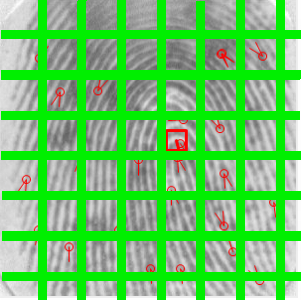
\includegraphics[angle=0,scale=1]{img/fingerprint_with_crate.jpg}
	\caption{Przykładowa siatka kodowa na tle odcisku}
	\label{simple_finger_crate_code}
    \end{center}
\end{figure}
\newline
Na ilustracji \ref{simple_finger_crate_code} można zauważyć fragmenty "kratki w której zmieściły się dwie minucję", po otrzymaniu kodu informacja ta zostanie stracona i silnik porównujący nie będzie 
wiedział czy w kratce była jedna czy więcej minucji. Rzeczywiste porównanie uwzględnia wartości kątów minucji leżących w tym samym kwadracie i dopiero na jej podstawie stwierdza zgodność.

\begin{figure}[hbt]
    \begin{center}
	
\includegraphics[angle=0,scale=1]{img/simple_crate_code.jpg}
	\caption{Otrzymany kod}
	\label{simple_code}
    \end{center}
\end{figure}
Na rysunku \ref{simple_code} pokazano otrzymany kod, który dla odpowiedniej(stałej) kolejności odczytywania utworzy binarny kod zer i jedynek.

\subsubsection{Ocena przydatności}
\begin{enumerate}
\item Zalety rozwiązania
\renewcommand*{\labelitemi}{\bullet}
\begin{itemize}
\item prostota algorytmu
\item kod odcisku zajmuje bardzo mało pamięci
\item XOR jako funkcja porównująca kody
\item bardzo niska złożoność obliczeniowa
\end{itemize}
\item Wady rozwiązania
\renewcommand*{\labelitemi}{\bullet}
\begin{itemize}
\item utrata informacji o minucji w przypadku za dużych podprzestrzeni
\item wrażliwość na przekształcenia
\item niska, wręcz zerowa skuteczność porównywania odcisków
\item wysoka wrażliwość na odciski o bardzo dużej liczbie minucji
\end{itemize}
\end{enumerate}

\vspace{.5cm}\par

Reasumując rozwiązanie tego typu nie można w żadnym stopni nazywać biometrią, zastosowane zostało jedynie jako wprawka dla następnych wersji algorytmu kodującego.
Ponieważ algorytm jest nieskuteczny należy zastanowić się nad przyczynami jego wad. Po pierwsze utratę informacji o minucjach zlokalizowanych w tej samej podprzestrzeni można zniwelować poprzez dodanie 
jeszcze jednego wymiaru do kodu, kąta pomiędzy styczną do grzbietu\footnote{przyjmuje się, że czarne części linii papilarnych nazywane są grzbietami białe dolinami} a osia odciętych. Oczywiście może zdarzyć się, że
minucje początkowo znajdujące się w tej samej podprzestrzeni nawet po dodaniu trzeciej współrzędnej dalej będą się w niej znajdować lecz prawdopodobieństwo to jest mniejsze. Świadczyć o tym może fakt iż
nagromadzenia minucji często znajdują się w miejscach gdzie linie papilarne zakręcają, tworząc pętle i wiry. Kąty tych minucji powinny być zupełnie inne. Rozwiązanie to zapobiega również błędnym 
porównaniom odcisków o dużej liczbie minucji. Odciski takie często mają rozkład minucji powodujący "zakodowanie" większości podprzestrzeni. Sytuacja ta jest na tyle uciążliwa, że dla pewnych wielkości siatki
dowolne dwa odciski były zaznaczane jako pochodzące od tej samej osoby. Dodanie kąta jako trzeciej wartości w kodzie nieco rozprasza zakodowanie. Kolejnym problemem jest wysoka wrażliwość na przekształcenia,
rozwiązaniem było zastosowanie sztucznych przekształceń obrazu i kodowanie wszystkich uzyskanych obrazów. Tworzy się w ten sposób wiele kodów dla jednego odcisku. Wszystkie te rozwiązania mają na celu 
polepszenie skuteczności algorytmu.

\subsection[Algorytm Kodujący][Macierz kodów]{Macierz kodów} 
Opisywany poniżej algorytm jest ulepszoną wersja naiwnego kodowania, eliminującą podstawowe wady pierwszego rozwiązania. Algorytm polega na kodowaniu kolejnych transformacji obrazu odcisku. Transformacje polegają na 
wykonaniu translacji obrazu o sprecyzowane wektory, oraz obracanie 
obrazu dla każdej translacji. Nieruchoma pozostaje ramka w której znajduje się wzorcowy obraz. Minucje które po transformacji znajdują się poza ramką są pomijane. Symuluje to uzyskanie odcisku poprzez 
inne przyłożenie palca do czytnika. Dla każdej otrzymanej transformacji obrazu wejściowego tworzony jest naiwny kod. Przykładowa transformacja obrazu pokazana jest na rysunku \ref{angle_shift} Wynikowym 
kodem odcisku jest sklejenie wszystkich otrzymanych kodów i liczba segmentów kodu czyli liczba translacji wykonanych na obrazie. W praktycznym zastosowaniu nie stosuje transformacji obrazu a jedynie listy 
minucji. W przypadku porównywania stosowana jest zasada wzorzec-próbka. Jeden z odcisków traktowany jest jako odcisk o większej jakości niż drugi, dla niego tworzony jest wyłącznie naiwny kod. Ma to 
odzwierciedlenie w pobieraniu próbek biometrycznych z reguły jest tak, że nad procesem pobierania próbki czuwa osoba odpowiedzialna za system,  odcisk powinien być pobrany poprawnie tak aby był jak 
najlepszej jakości. Drugi odcisk pochodzi z systemu nad którym nikt nie czuwa, dla niego tworzona jest macierz kodów. Dokładnie jak w zastosowaniu codziennym użytkownik systemu proszony jest(najczęściej 
przez automat) o przyłożenie palca do skanera w celu pobrania próbki. Nie ma żadnej gwarancji iż poprawnie złoży próbkę. Założenie to odzwierciedla warunki rzeczywiste pozyskiwania odcisków. Następnym 
krokiem jest porównanie odcisku. Algorytm bierze kod wzorca i porównuje ze wszystkimi 
naiwnymi kodami macierzy kodów. 
\par 
Porównując pojedyncze kody możliwe są trzy przypadki porównań
\renewcommand*{\labelitemi}{\bullet}
\begin{itemize}
\item \textbf{1 : 1} dopasowanie, elementy wzorca są zgodne z próbką
\item \textbf{1 : 0} niedopasowanie wzorca, element wzorca nie istnieje w próbce
\item \textbf{0 : 1} niedopasowanie próbki, element próbki nie istnieje we wzorcu
\end{itemize}
\vspace{.5cm}\par
Wybierany jest najlepszy wynik porównania tzn. taki dla którego liczba porównań 1:1 jest największa. Jako wskaźnik stosowano również
minimalizację liczby niedopasowań wzorca i próbki. Niestety dla takich wymagań algorytm wybierał taką transformację dopasowanego obrazu próbki dla której większość minucji znajdowała się poza ramką obrazu, czyli były pomijane.
Ubocznym skutkiem poprawienia wskaźnika było zmniejszanie liczby porównywanych minucji. Zaburza to rzeczywiste porównywanie kodów.
\begin{figure}[h]
    \begin{center}
	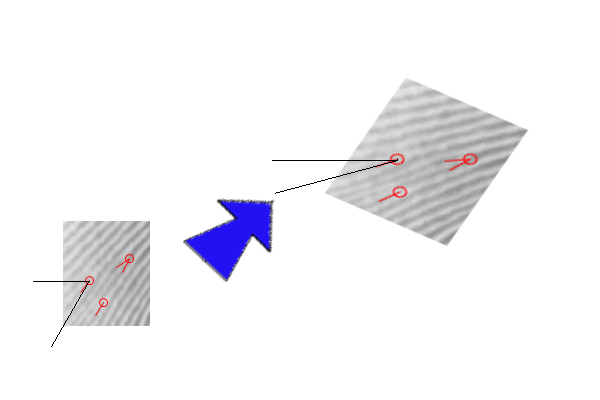
\includegraphics[angle=0,scale=.6]{img/angle_shift.jpg}
	\caption{W trakcie transformacji należy wyliczyć nowe wartości kątów}
	\label{angle_shift}
    \end{center}
\end{figure}

Istotny wpływ na jakość porównania ma wielkość kodu czyli ilość i dokładność informacji w nim przechowywanych. Wielkość kodu musi być dobrana w taki sposób aby dopasowanie było w miarę poprawne i 
jednocześnie ilość obliczeń potrzebnych do porównania nie była zbyt duża. Na wielkość kodu składa się wielkość naiwnego kodu oraz ilość segmentów.

\begin{table}
\begin{tabular}{l l p{13cm}}
\bullet & SC_{size} &  rozmiar naiwnego kodu \\
\bullet & SEG_{size} & ilość segmentów kodowych \\
\bullet & MC_{size} & rozmiar macierzy kodów \\
\bullet & X_{cres} & szerokość (w pikselach) obrazu z odciskiem \\
\bullet & Y_{cres} & wysokość (w pikselach) obrazu z odciskiem \\
\bullet & A_{cres} & zakres kąta(podawany w stopniach) obrazu z odciskiem\\
\bullet & A_{res} & wartość kąta(podawana w stopniach) o jaką maksymalnie należy obracać obraz\\
\bullet & C_{sep} & rozmiar kratki kodu \\
\bullet & X_{step} & odstęp w poziomie pomiędzy najbliższymi translacjami obrazu \\
\bullet & Y_{step} & odstęp w pionie pomiędzy najbliższymi translacjami obrazu \\
\bullet & COV_{step} & wskaźnik odstępu pomiędzy najbliższymi translacjami podawany jako wielokrotność kratki kodu \\
\bullet & A_{step} & odstęp kątowy pomiędzy najbliższymi obrotami obrazu\\
\end{tabular}
\end{table}

\begin{equation}
SC_{size}=[ \frac{X_{cres}}{C_{sep}}] * [ \frac{Y_{cres}}{C_{sep}}]* [ \frac{A_{cres}}{A_{sep}}]\qedhere \\
\label{eq:SC_size}
\end{equation}

\begin{equation}
X_{step}=[ X_{cres} * COV_{step}]
\label{eq:x_step}
\end{equation}

\begin{equation}
Y_{step}=[ Y_{cres} * COV_{step}]
\label{eq:y_step}
\end{equation}

\begin{equation}
SEG_{size}=[ \frac{X_{cres}}{X_{step}}] * [ \frac{Y_{cres}}{Y_{step}}] * [2*\frac{A_{res}}{A_{step}}] \qedhere \\
\label{eq:SEG_size}
\end{equation}

\begin{equation}
MC_{size}=SEG_{size}*SC_{size} \qedhere \\
\label{eq:MC_size}
\end{equation}

\subsubsection{Przykład 1}
Dla obrazu o wymiarach [300 x 300 x 300], rozmiarze kratki kodu [25 x 25 x 30], wskaźniku odstępu 0.5 i odstępie kątowym 15$^\circ$ i maksymalnym kącie obroty 45$^\circ$ otrzymano kod o 
2500 segmentów o wielkości jednego segmentu 1440 bitów(0,175kB) co daje razem 3600000 bitów(0,429Mb). 

\subsubsection{Ocena przydatności}

\begin{enumerate}
\item Zalety rozwiązania
\renewcommand*{\labelitemi}{\bullet}
\begin{itemize}
\item prostoty algorytm kodujący
\item eliminuje podstawowe wady naiwnego kodu
\item skuteczniejszy niż naiwny kod
\item łatwość konfiguracji
\end{itemize}
\item Wady rozwiązania
\renewcommand*{\labelitemi}{\bullet}
\begin{itemize}
\item utrata informacji o minucji w przypadku za dużych podprzestrzeni
\item wrażliwość na przekształcenia nieliniowe
\item średnia skuteczność porównywania odcisków
\item duży rozmiar kodu ( większy niż $2^{21}$ mniejszy niż $2^{22}$)
\item brak trywialnej funkcji porównującej kody
\end{itemize}
\end{enumerate}
\vspace{.5cm}\par

Mimo, iż kolejna wersja algorytmu jest lepsza od poprzedniej wciąż nie jest pozbawiona wad. Podobnie jak w poprzednim rozwiązaniu za duży rozmiar kratki kodowej może zniekształcać informacje i prowadzić do 
zbytniego uproszczenia kodu. Duża kratka może obejmować więcej niż jedną minucje. Z drugiej strony zbyt mały rozmiar kratka może prowadzić do zmniejszenia skuteczności algorytmu. Reprezentacja minucji jako 
otoczenia w którym się znajduje ma symulować zniekształcenia obrazu powstałe w procesie pobierania próbki biometrycznej. Należy uzyskać kompromis pomiędzy tolerancją na zniekształcenia, a skutecznością 
dopasowania. Prostą zależność pokazują schematyczne wykresy \ref{img:crate_size}. Algorytm nie jest odporny na przekształcenia nieliniowe. W procesie pobierania próbki biometrycznej zniekształcenia takie 
jak spłaszczanie palca nie musi dotyczyć całej jego powierzchni, nie musi też być równomierne. Algorytm stara się kompensować zniekształcenia poprzez wskazywanie jedynie otoczenia w którym znajduje się 
minucja, a nie jej dokładnego położenia. Dlatego tak istotny jest właściwy dobór wielkości kratki kodu. Przekształcenia mające symulować pobranie próbki w inny sposób niż w procesie rejestracji są 
wykonywane na całym obrazie. Nie trudno się domyśleć, iż może istnieć takie zniekształcenie obrazu którego nie będzie dało się dopasować do wzorca poprzez obroty i przesunięcia całego obrazu. rozwiązaniem 
tego problemu byłoby wprowadzenie przekształceń na fragmentach obrazu, zamiast na całości. Wiąże się to ze sporym wzrostem rozmiaru kodu. Rozwiązanie to nie zostało zastosowane. Skuteczność porównywania 
znacząco wzrosła w porównaniu do poprzedniej metody, szczegółowe wyniki przedstawione są w rozdziale 4. Kolejną wadą jest znaczny wzrost rozmiarów kodu. Rozwiązaniem może być analiza wyglądu kodu. Kod 
odcisku można porównać wyglądem do macierzy rzadkich. Składa się głownie z "0", gdzieniegdzie występują "1". Dlatego można zastosować prostą kompresje zapisując jedynie położenie "1" domyślnie pozostałe 
miejsca w kodzie są "0". Jednak w dobie szybko rozwijającej się techniki i ciągłego postępu pamięć dyskowa jest raczej tania i nie powinno się przejmować obszernością zaproponowanego rozwiązania. 
Zwłaszcza, że baza danych dla jednego wzorca przechowuje jedynie naiwny kod, a nie jego macierz kodów, macierze są tworzone jedynie dla próbek i są przechowywane przez pamięć operacyjną w trakcie 
porównywania. 
\subsubsection{Przykład 2\footnote{Wyniki dotyczą danych podanych w przykładzie 1}}
Baza danych 1 mln wzorców zajmuje 171,66 MB. Gdyby zaszła potrzeba przechowywania macierzy kodów zamiast naiwnego kodu baza zajmowałaby 419,09 GB. 
\subsubsection{Przykład 3\footnotemark[\value{footnote}]}
Algorytm stwierdzając podobieństwo porównuje naiwny kod wzorca z macierzą kodów próbki, porównując każdy element wzorca z odpowiadającym elementem próbki w każdym jej segmencie. W trakcie całego procesu 
algorytm wykonuje 3600000 porównań.
\vspace{.5cm}\par
Jak widać duży rozmiar kodu nie wpływa znacząco na zdolność magazynowania go w bazach danych, natomiast istotny jest w procesie porównywania. Wraz ze wzrostem skomplikowania funkcji kodującej wzrósł 
stopień skomplikowania funkcji porównującej kody. Utrudnienie polega na porównywaniu kodu wzorca z każdym segmentem kodu próbki. Porównanie to podobnie jak w początkowej wersji algorytmu może być wykonane 
funkcją XOR. Zmiana polega na tym, że algorytm spośród wszystkich porównań musi wybrać takie dla którego wystąpiło najwięcej dopasowań (1 : 1). Poniżej przedstawiono schematycznie wpływ wielkości kratki kodu na poprawność i łatwość dopasowania kodów.
\begin{figure}[h]
    \begin{center}
	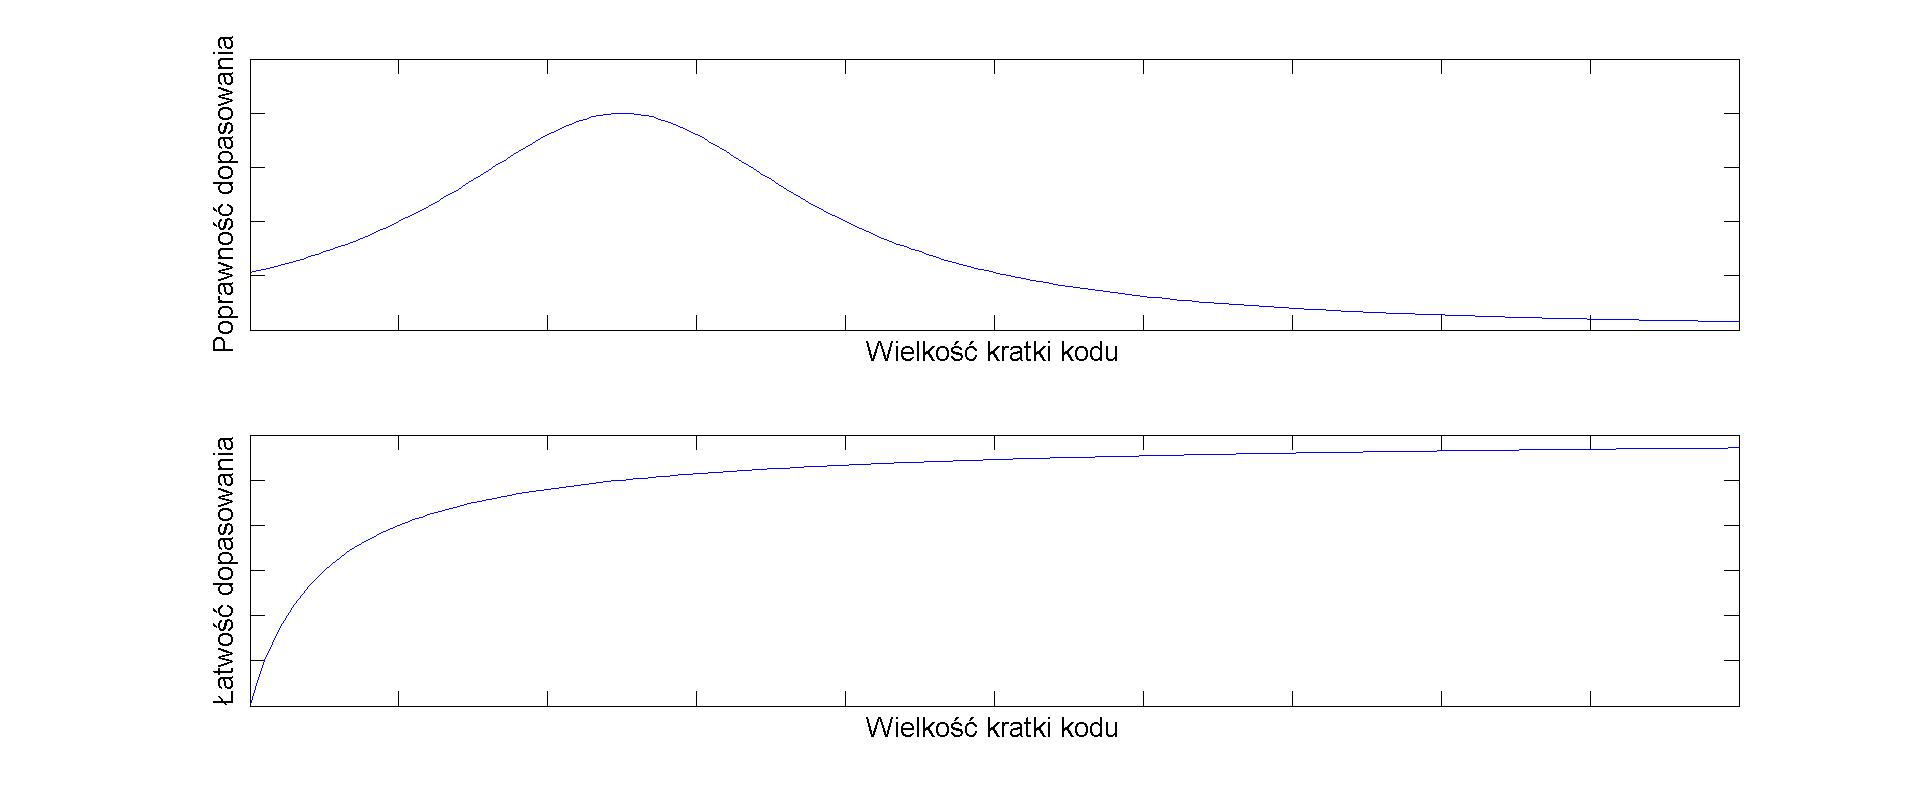
\includegraphics[angle=0,scale=.25]{img/crate_size.jpg}
	\caption{Wpływ wielkości kratki kodu}
	\label{img:crate_size}
    \end{center}
\end{figure}

\section[Przyczyny zastosowań kodu odcisku][Przyczyny zastosowań kodu odcisku]{Przyczyny zastosowań kodu odcisku}

W obecnie istniejących systemach biometrycznych wykorzystujących odcisk palca przeważają metody minucyjne. Jako sposób porównywania obrazów stosowane jest podejście obiektowe. Ideą tej pracy jest 
sprawdzenie możliwości zastosowanie prostego kodowania i odejścia od obiektowego sposobu porównywania odcisków. Praca stara się sprawdzić czy utrwalony model obiektowy o zmiennej liczbie obiektów można 
zastąpić kodem o stałej długości. Weryfikację odcisków można przeprowadzić za pomocą prostej funkcji porównującej. Gdyby rozwiązanie takie wprowadzono w życie, silnik liczący mógłby zostać przeniesiony na 
karty i urządzenia mobilne o ograniczonej mocy obliczeniowej. Weryfikacja mogła by przebiegać bezpośrednio na kartach przenoszonych przez użytkowników. Dodatkowym atutem metody jest pośrednie kodowanie 
informacji biometrycznej. Niepożądane zdobycie kodu odcisku powinno uniemożliwić odtworzenie obrazu lub listy minucji, bez posiadania wiedzy o algorytmie kodującym. Algorytm niekoniecznie musi zapisywać 
położenie minucji w tak prosty sposób jak w przedstawionym powyżej rozwiązaniu. Zawsze możliwe jest dołożenie kilku fałszywych minucji do kodu i zapamietaniu ich położenia. Kolejnym możliwym sposobem 
zabezpieczenia jest odrzucanie wyników zbyt zgodnych. Osoba posiadająca skradziony kod odcisku nie będzie miała możliwości weryfikacji używając skradzionego kodu wzorca. System z łatwością stwierdzi 100\% 
zgodność i z będzie mógł odrzucić próbę fałszerstwa. Dowolne modyfikacje na kodzie w celu wprowadzenia zakłóceń do skradzionego kodu powinno uniemożliwić poprawną weryfikację. Niestety metoda nie jest \
pozbawiona wad. Szczegółowe wyniki działania przedstawiono w rozdziale 4.


\chapter{Porównanie wyników algorytmu z komercyjnym rozwiązaniem} 

Systemy biometryczne powinny cechować się dużą skutecznością porównań odcisków, a czas potrzebny na porównanie odcisków powinien być jak najszybszy. Dlatego systemy należy oceniać biorąc pod uwagę właśnie te kryteria. Jakość obu cech jest bardzo istotna. Szybko działający system, dla którego EER\footnote{\em ang. Error equality rate, błąd zrównoważony - błąd, dla progu, dla którego błąd fałszywych odrzuceń i błąd fałszywych dopasowań jest taki sam} jest wysoki jest tak samo nieskuteczny jak bezbłędny system, który obliczenia prowadzi zbyt długo. Ten ostatni można wykorzystać jako wsparcie dla daktyloskopii\footnote{z gr. daktylos – palec i skopeo – patrzę, oglądam) – technika śledcza zajmująca się badaniami porównawczymi linii papilarnych}. Ocena rozwiązania podawana jest na tle komercyjnego programu Fingers Identification Technology\footnote{SDK do porównywania odcisków na licencji Neurotechnology}. Dla potrzeb tej pracy użyto 30 dniowej wersji demonstracyjnej. W zależności od metody porównującej zmieniany jest sposób dopasowywania minucji. Domyślnie SDK posiada swoje wskaźniki obliczające stopień dopasowania, aby porównywanie było miarodajne wykorzystuje ten program jedynie do ekstrakcji minucji i zwrócenia liczby dopasowanych i niedopasowanych minucji. 
\section[Analiza statystyczna kodu][Analiza statystyczna kodu]{Analiza statystyczna kodu} 
Typowym sposobem oceny biometrycznych systemów używających kodowania jako sposobu przetwarzania informacji jest badanie właściwości statystycznych kodu. Dlatego też przeprowadzono porównania w dwóch grupach. Pierwsza z nich dotyczy porównania między odciskami pochodzącymi od tego samego palca. Druga grupa to porównania między różnymi odciskami. W przypadku analizy algorytmu wykonano 2800 porównań. Porównywania wykonywano na zbiorze 800 odcisków, pochodzących od 100 różnych palców, gdzie każdy palec posiada 8 pobranych od niego odcisków. Wybrano dużą liczbe odcisków aby możliwie najlepiej sprawdzic działanie algorytmu. Test wykonywany poprzez porównywanie każdy z każdym wewnątrz odcisków pochodzących od tego samego palca. Druga grupa dotyczy porównania między odciskami pochodzącymi od różnych palców. W przypadku analizy algorytmu wykonano 4950 porównań. Test wykonano na zbiorze 100 odcisków. W tym porównaniu zmniejszono liczbę odcisków, ponieważ nie porównywano odcisków pochodzacych od tego samego palca. Liczba 100 odcisków wystarczyła do wykonania zadowalającej liczby porównań. Jednocześnie mniejsza liczba odcisków jest niewiarygodna dla takiego testu. Porównania wykonano poprzez porównanie każdy - z każdym wewnątrz odcisków pochodzących od różnych palców. Analogiczne testy wykonano dla SDK Neurotechnology. Porównując te same odciski wykonano 300 porównań dla odcisków pochodzących od tego samego palca i 300 dla odcisków pochodzących od różnych. Mała liczba porównań świadczy o tym iż uznano komercyjny program za dość powtarzalny, a testy wykonano dla zgromadzenia wyników na wspólnej bazie odcisków.
\subsection{Rezultaty testów}
\begin{figure}[!hb]
    \begin{center}
		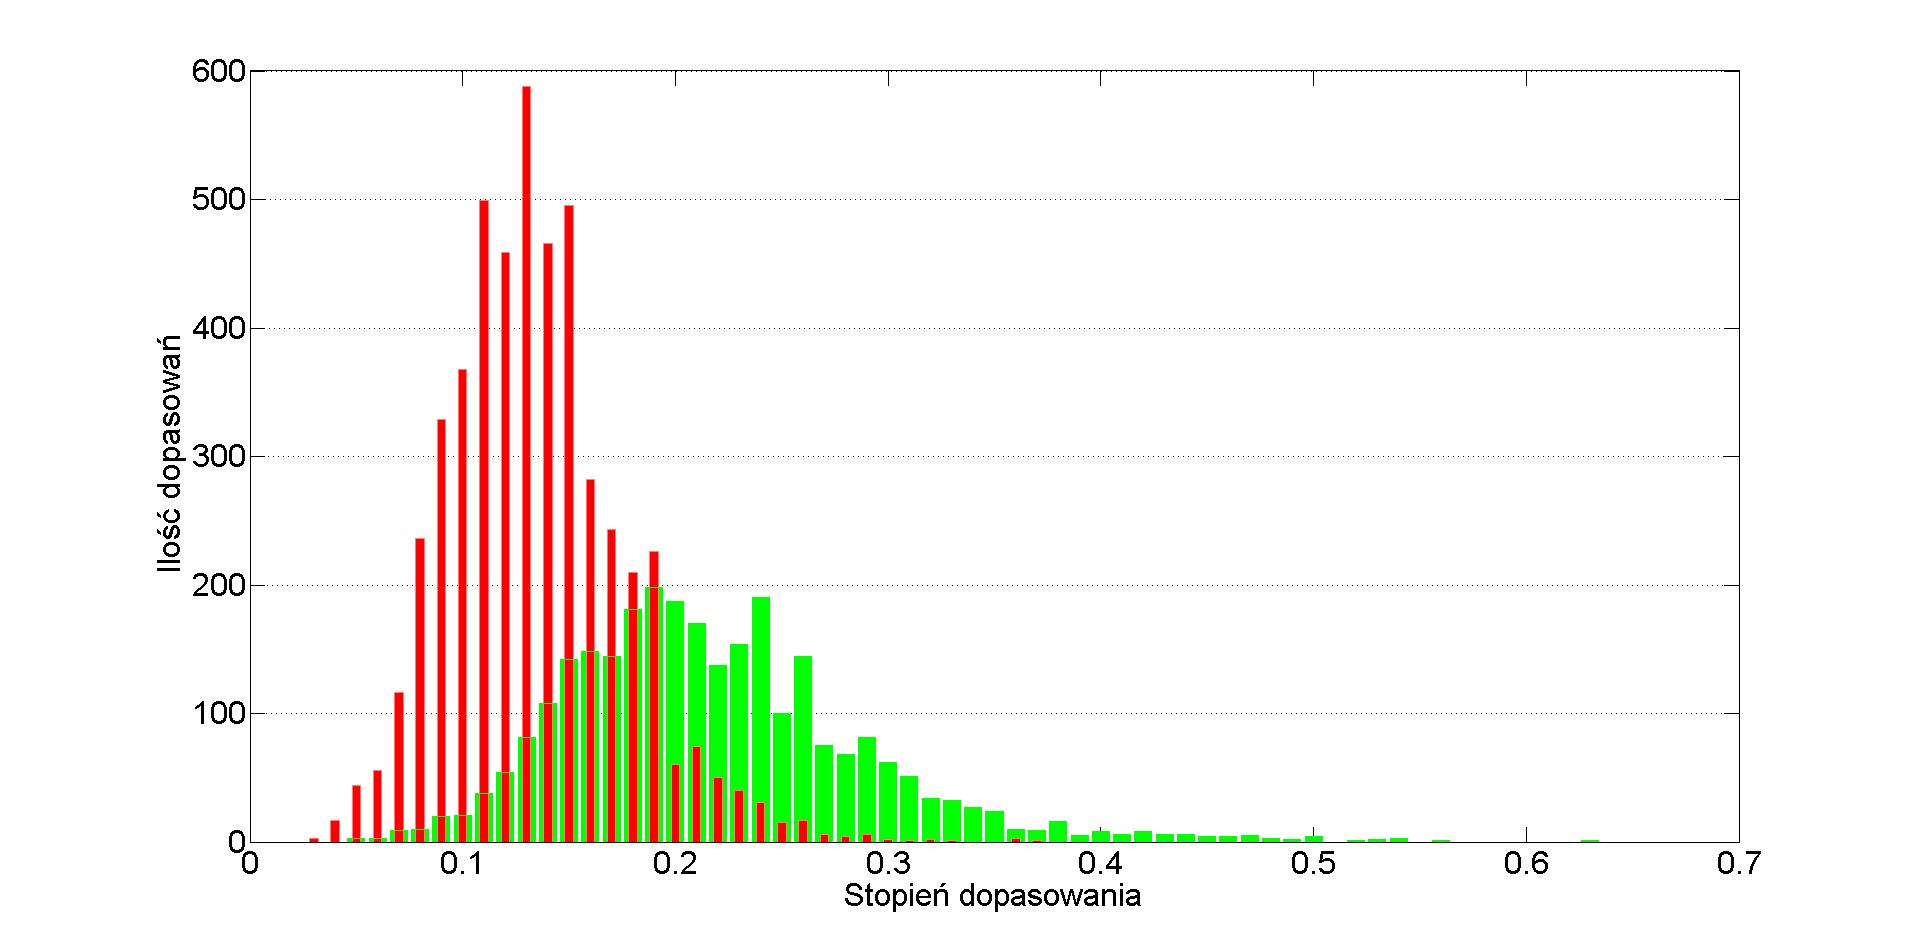
\includegraphics[angle=0,scale=0.27]{img/pattern_bar_statistic_analyses_code_way.jpg}
		\caption{Ilość dopasowań w zależności od jakości dopasowania do odcisku wzorca (test Algorytmu kodowego)}
		\label{img:code_stat_bar_pattern}
    \end{center}
\end{figure} 
Rysunek\ref{img:code_stat_bar_pattern} przedstawia porównania wewnątrz tych samych i różnych odcisków. Kolorem zielonym zaznaczono porównania w grupie tych samych odcisków, czerwonym wewnątrz różnych. Na osi odciętych zaznaczono stopień dopasowania. Jest to iloraz ilości porównań 1:1 do ilości minucji we wzorcu. Świadomie nie stosowano tu klasycznego podejścia odległości Hamminga\footnote{ang. Hamming distance – w teorii informacji jest to wprowadzona przez Richarda Hamminga miara odmienności dwóch ciągów o takiej samej długości}, ponieważ utworzony kod odcisku ma głównie "0", "1" czyli minucje występują w nim rzadko. Zastosowanie odległości Hamminga dawało by wysoką zgodność kodów dla porównywania w obu grupach i wynik byłby nieczytelny. Na osi rzędnych zaznaczono ilość takich dopasowań. Dla czytelności wykres \ref{img:code_stat_line_pattern} przedstawia liniowy sposób reprezentacji poprzedniego wyniku. W dalszej części przedstawiono tylko rysunki liniowe. Wyraźnie widać iż rejony kreślone przez funkcje porównań tych samych i różnych odcisków pokrywają się(miejscie przecięcia zostało zaznaczone niebieską linią). Punk ten wykorzystywany jest do obliczania wskaźników FAR i FRR. Oznacza to, że metoda nie jest pozbawiona błędu. Istnieją odciski które zostaną błędnie zaklasyfikowane jako poprawne oraz te które zostaną błędnie odrzucone. EER dla takiej metody wynosi około 17\%. Oznacza to że przy wyborze progu zaznaczonego niebieską linią co piąte porównanie zostanie błędnie sklasyfikowane. Innowacyjność tej metody porównywania odcisków wskazywałaby na to, że metoda nie koniecznie powinna działać rewelacyjnie. Wynik w granicach 17\% jest jednak wynikiem niedopuszczalnym i przekreśla jakąkolwiek użyteczność tej metody. Dla przedstawionego progu FAR\footnote{ang. False Acceptance Rate -błąd fałszywej akceptacji, ilość odcisków błędnie sklasyfikowanych jako prawdziwe do całości porównywanych odcisków przez system} wynosi nieco ponad 11\%, wiec ok. co dziesiąty odcisk oszusta zostanie zaakceptowany jako prawdziwy. W ustalonym progu FRR\footnote{ang. False Rejection Rate -błąd fałszywego odrzucenia, ilość odcisków błędnie sklasyfikowanych jako nieprawdziwe do całości porównywanych odcisków przez system} wynosi ponad 23\%, oznacza to, że prawie co czwarty prawidłowy odcisk będzie odrzucony. Błąd ten może nie prowadzi do akceptacji próby włamania ale może być uciążliwy dla właściwych użytkowników. Wyobraźmy sobie sytuacje, że ten system zainstalowano w jednym z bankomatów. Więc średnio co 4 wypłata pieniędzy będzie niemożliwa bo system odrzuci nasze logowanie i cały proces należy powtórzyć. Sytuacja wygląda znacznie gorzej gdy system ma zapewniać zerowy błąd akceptacji, wtedy błąd fałszywego odrzucenia wynosi ponad 96\%. Rysunek \ref{img:code_stat_line_sample} pokazuje te same wyniki dla porównywania na tle próbki. Podobnie jak poprzednio wynik do ilość porównań 1:1 do ilości minucji w próbce. Współczynnik EER wzrósł a współczynniki ZERO FRR i ZERO FARi różnią  nieznacznie. Większe różnice występują na poziomie FAR i FRR. Wynika to ze sposobu porównywania odcisków przez algorytm. W skutek dopasowywania kodów algorytm dokręca obrazy odcisków tak aby liczba porównań 0:1 I 1:0 była najmniejsza. Skutkiem ubocznym jest zmniejszanie ilości rozpatrywanych minucji po stronie próbki, dzięki temu liczba rozpatrywanych minucji w próbce jest generalnie mniejsza od liczby minucji we wzorcu. Zmniejszenie ilości minucji po stronie próbki zmniejsza FRR i zwiększa FAR. Dzieje się tak, ponieważ ta sama liczba dopasowanych minucji dzielona przez mniejsza liczbę rozpatrywanych minucji w próbce powoduje przesuwanie wykresu ku większym wartościom. Efekt ten dotyczy zarówno porównań wśród tych samych jak i różnych odcisków, a ponieważ porównania dla odcisków różnych mają mniejszą liczbę trafień niż dla tych samych wykres wykres ten szybciej przesunął się w prawą stronę, a wraz z nim próg EER. Zjawisko to nie występuje dla testów aplikacji $Neurotechnology$ wynika to z innego algorytmu dopasowującego minucje.
\begin{figure}[!ht]
    \begin{center}
		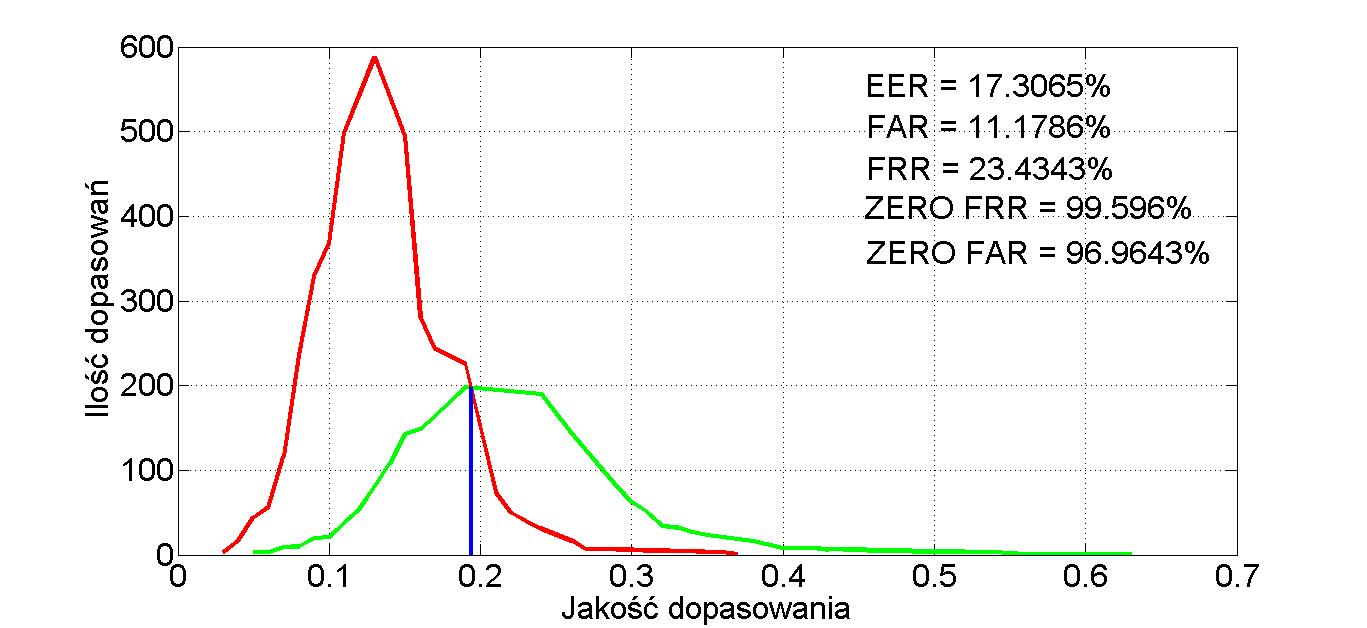
\includegraphics[angle=0,scale=0.27]{img/pattern_line_statistic_analyses_code_way.jpg}
		\caption{Ilość dopasowań w zależności od jakości dopasowania do odcisku wzorca (test Algorytmu kodowego)}
		\label{img:code_stat_line_pattern}
    \end{center}
\end{figure} 

\begin{figure}[!htb]
    \begin{center}
		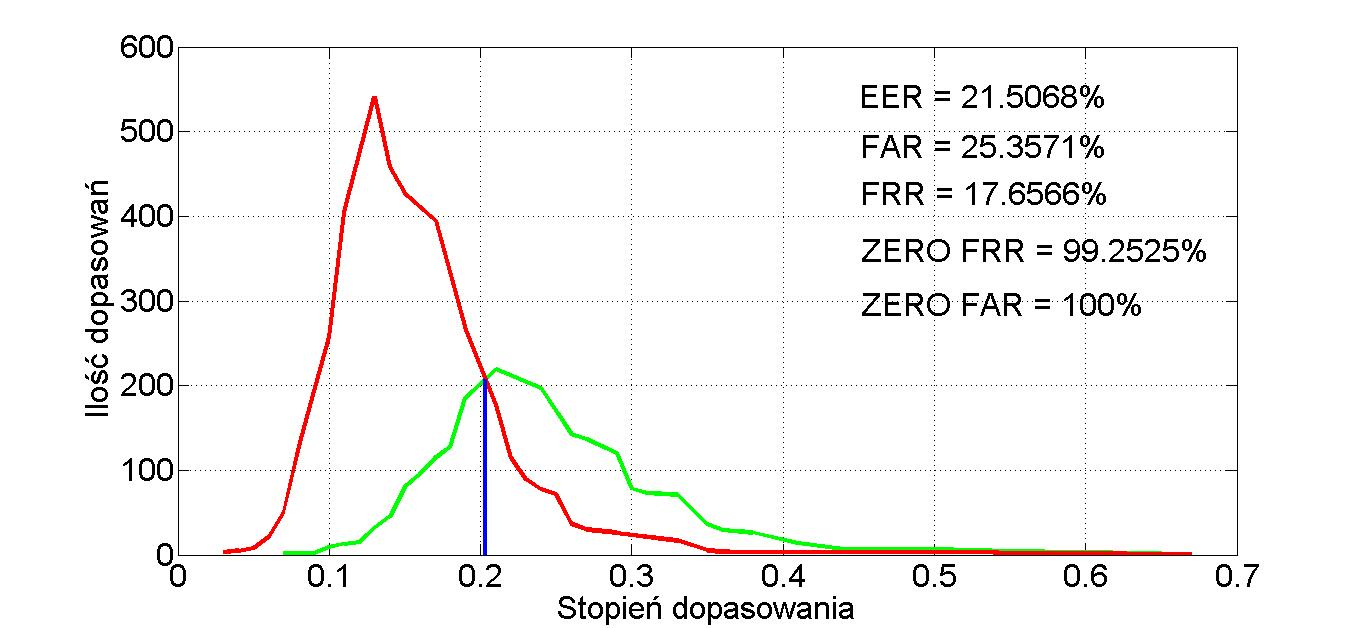
\includegraphics[angle=0,scale=0.27]{img/sample_line_statistic_analyses_code_way.jpg}
		\caption{Ilość dopasowań w zależności od jakości dopasowania do odcisku próbki (test Algorytmu kodowego)}
		\label{img:code_stat_line_sample}
    \end{center}
\end{figure} 
Wyniki przedstawione na tle odcisków próbki są nieznacznie gorsze od wyników przedstawianych na tle wzorca. Wynika to z tego, że algorytm szukając najlepszego dopasowania stosuje transformacje na obrazie próbki, w zależności od dokonanego przekształcenia liczba minucji biorących udział w porównaniu się zmienia mniejsza liczba niedopasowanych minucji może być spowodowana zmniejszeniem się liczby rozpatrywanych minucji próbki. Jest to negatywny skutek uboczny minimalizacji porównań 1:0 i 0:1.
\vspace{.5cm}\par
Komercyjne rozwiązanie wykorzystano w taki sposób aby algorytm porównujący miał zbliżone działanie do przedstawianego kodowania. Wykorzystano jedynie liczbę minucji dopasowanych i nie dopasowanych, generując takie same wykresy. Kolory na wykresach są takie same jak dla testów kodu. Zastosowane metoda nie sugeruje się wskaźnikiem dopasowania zwracanym przez program $Neurotechnology$. Algorytm komercyjny nie korzysta z kodowania odcisku. Wszelkie dopasowania odbywają się przez porównywanie obiektów, a nie kodów. Algorytm komercyjny ma przewagę nad kodowym rozwiązaniem, przechowuje informacje o typie minucji oraz buduje siatkę łącząc dopasowywane minucje. Jest to kolejna informacja, dodatkowo stwierdzająca zgodność dopasowania. Na rysunkach \ref{img:ob_stat_bar_pattern} i \ref{img:ob_stat_line_pattern} zaprezentowano analogiczne do poprzedniego testu wykresy jakości dopasowania względem odcisku wzorca. Rysunki \ref{img:ob_stat_bar_sample} oraz \ref{img:ob_stat_line_sample} prezentują te same wyniki dla próbki. 
\vspace{.5cm}\par
Dla $Neurotechnology$ wynik również nie jest pozbawiony błędu, choć jest o wiele lepszy niż w przypadku zastosowanego algorytmu kodującego. EER dla tej metody wynosi ok 1.5\%, mimo iż jest 10 krotnie mniejszy niż dla kodu odcisku,  nie zapewnia należytej ochrony wymaganej od systemów biometrycznych. Warto zauważyć, iż podawany wynik nie dotyczy skuteczności oprogramowania $Neurotechnology$, a jedynie jego udziału w proponowanym sposobie porównywania odcisków. Zdecydowanie lepiej wypadają też współczynniki FAR i FRR, które wynoszą odpowiednio ok 1\% i 2\%. Natomiast znacznie lepiej prezentuje się w przypadku błędów zerowych. Wystarczy zaakceptować błąd w granicach 7\% i system stanie się bezbłędny. Oczywiście wyniki dotyczą tylko bazy danych na której był przeprowadzany test. Przeprowadzany test dowodzi, iż kodowa metoda porównywania odcisków dopasowuje odciski znacznie gorzej niż metoda obiektowa. Dodatkowo porównywanie jedynie liczby minucji pasujących nie wystarcza do jednoznacznego stwierdzenia podobieństwa bądź niepodobieństwa obrazów. Kolejną wadą przedstawianego rozwiązania jest brak porównań dla których jest 100\% zgodność lub analogiczna niezgodność. Wynika to z doboru parametrów, a zwłaszcza wielkości kratki kodu. Zmniejszenie kratki powodowało pojawianie się porównań o 100\% niezgodności natomiast zwiększanie sprzyja łatwiejszemu dopasowywaniu kodów. Niestety ustawienia te źle wpływały na ilość poprawnych porównań. Ustawienie optymalnej wielkości kratki powoduje zmniejszenie liczby całkowitych zgodności i niezgodności.

\begin{figure}[!hbt]
    \begin{center}
		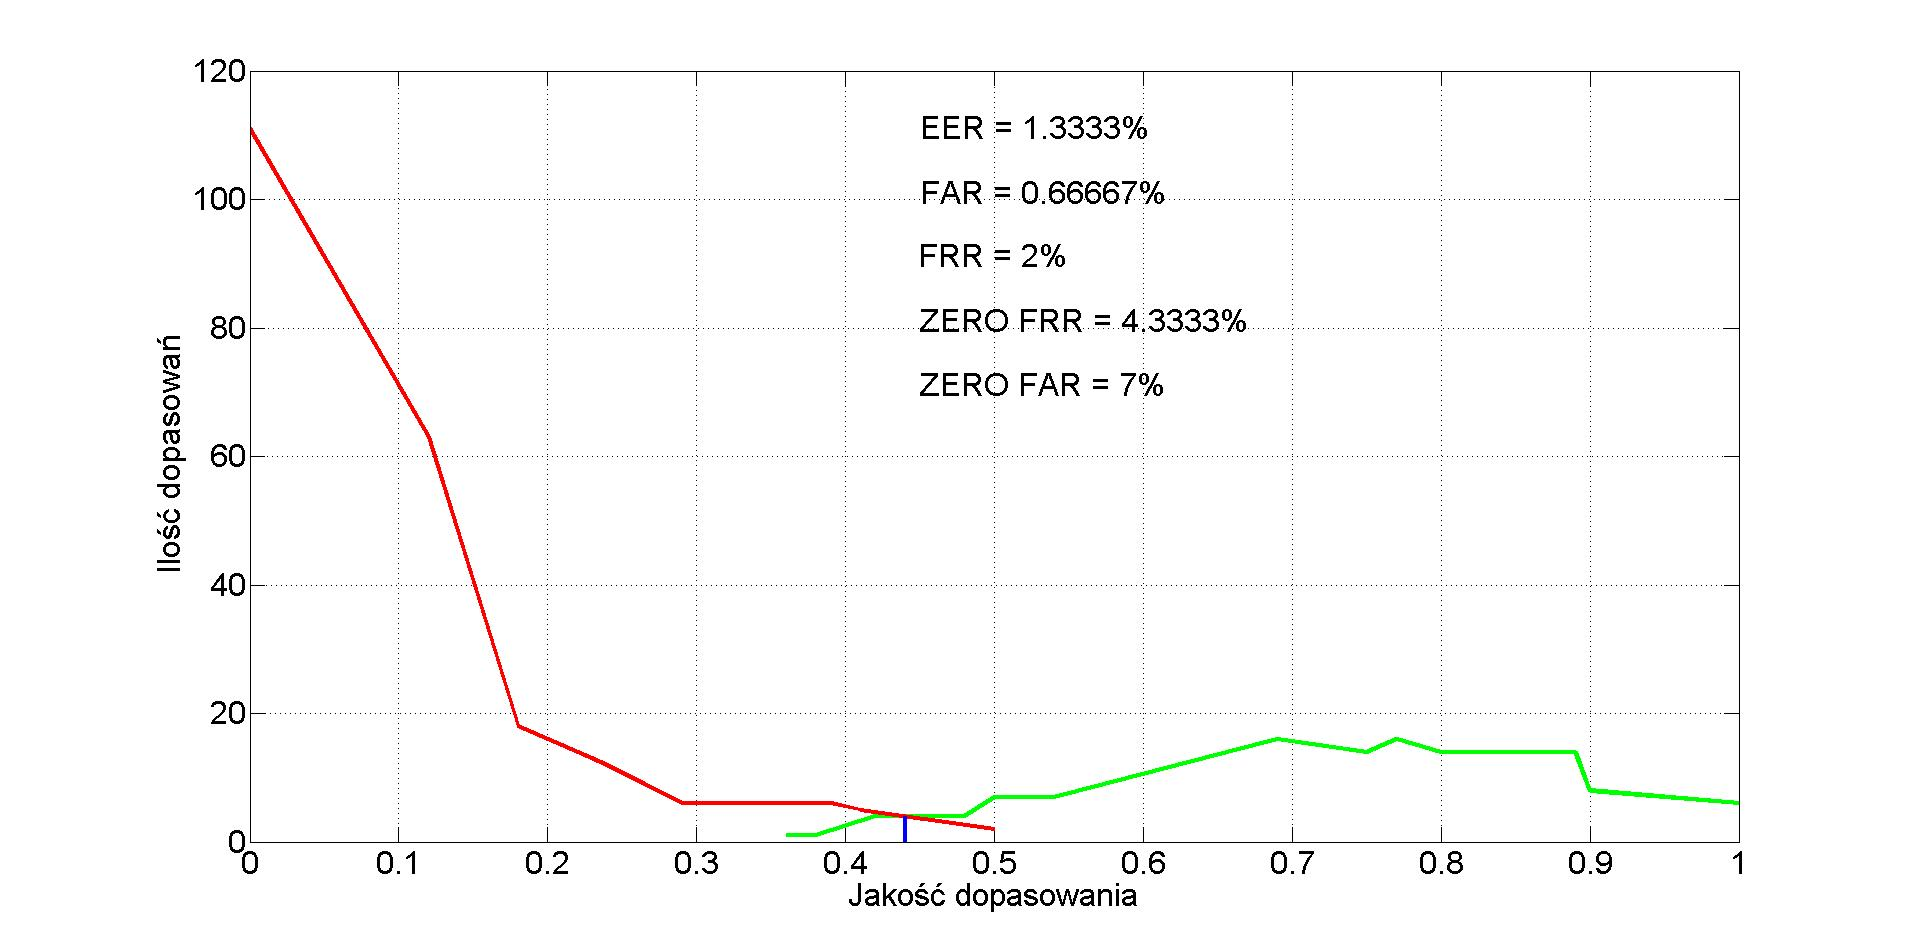
\includegraphics[angle=0,scale=0.27]{img/pattern_line_statistic_analyses_ob_way.jpg}
		\caption{Ilość dopasowań w zależności od jakości dopasowania do odcisku wzorca (test $Neurotechnology$)}
		\label{img:ob_stat_line_pattern}
    \end{center}
\end{figure} 
\newpage 

\begin{figure}[!hbt]
    \begin{center}
		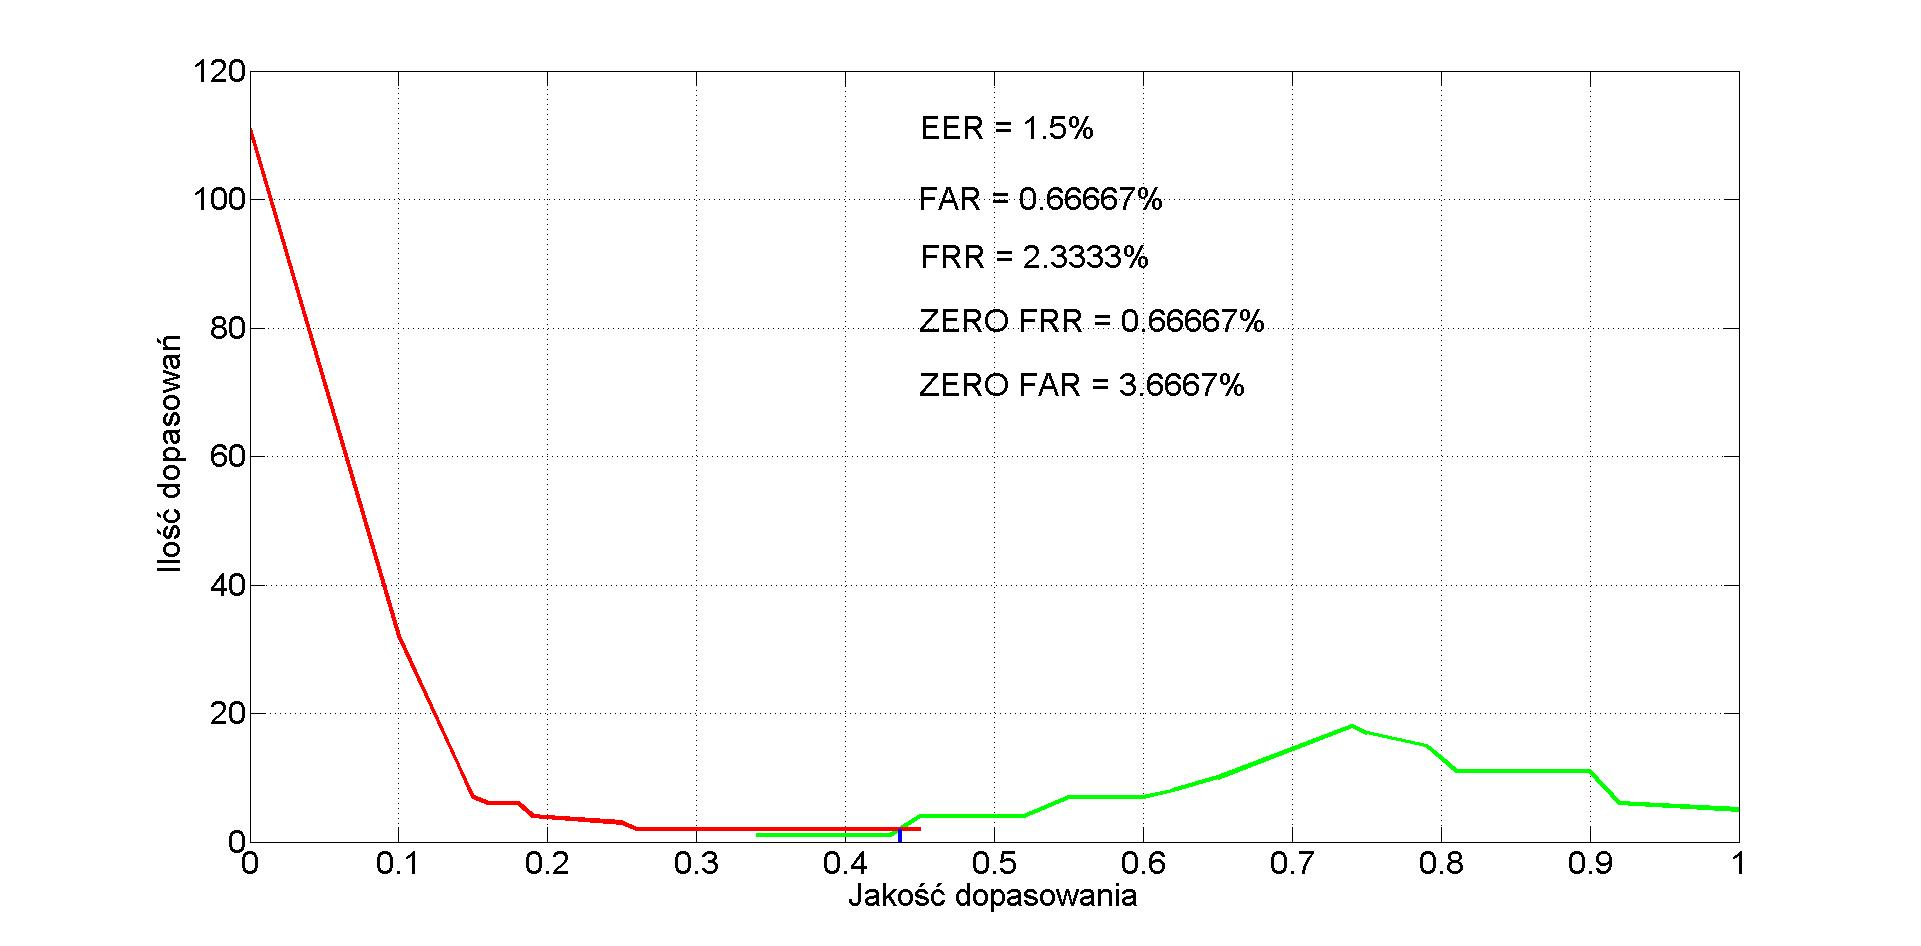
\includegraphics[angle=0,scale=0.27]{img/sample_line_statistic_analyses_ob_way.jpg}
		\caption{Ilość dopasowań w zależności od jakości dopasowania do odcisku próbki (test $Neurotechnology$)}
		\label{img:ob_stat_line_sample}
    \end{center}
\end{figure} 

\newpage 
\section[Rozkład punktów porównania][Rozkład punktów porównania]{Rozkład punktów porównania}

Przeprowadzone testy dowodzą jednoznacznie, że sposób porównywania tylko liczby zgodnych minucji nie wystarcza do stwierdzenia poprawnego podobieństwa lub nie podobieństwa obrazów. Choć metoda ta jest jedną z głównych metod stwierdzających prawidłowe dopasowanie odcisków to dla wykorzystań opisywanego algorytmu jest całkowicie zawodna. Przyczyn może być wiele
\renewcommand*{\labelitemi}{\bullet}
\begin{itemize}
\item Błąd algorytmu
\item Błąd implementacji
\item Niewystarczająca ilość kodowanej informacji
\item Zbytnie uproszczenie kodowanej informacji
\item Brak filtrowania minucji, chodzi tu o odrzucanie minucji o niewystarczającej jakości
\item Błąd sposobu porównania kodów
\end{itemize}
Przyczyny związane z błędami w kodzie programu odrzucam, gdyż testy aplikacji dowodzą prawidłową realizację wymyślonego algorytmu. Błąd algorytmu stawiałby poważną barierę w rozwoju tego typu podejścia dlatego dla celów badawczych również jest tu pomijany. Zwiększenie ilości kodowanej informacji mogłoby przekształcić algorytm kodowania w inny zapis algorytmu obiektowego. Naturalne wydaje się iż w algorytmach tworzących kod jakiejś próbki biometrycznej wartości cech biometrycznych są uśredniane i wynik ten nie powinien przeszkadzać w porównywaniu obrazów. Dowodem tego może być algorytm Dougman-a do kodowania tęczówki oka. Obraz tęczówki jest świadomie uśredniany, a mimo wszystko nie przeszkadza to w dalszej identyfikacji. trafnym pomysłem jest odrzucanie minucji o złej jakości. W procesie przetwarzania obrazu znalezione współrzędne niekoniecznie muszą wyznaczać minucje odcisku. Nikt nie gwarantuje wysokiej jakości obrazu z czytnika. Dlatego znalezione punkty mogą być tylko zakłóceniem obrazu a nie rzeczywistą minucją. Mimo tego rozwiązanie to nie zostało zastosowane. Powodem jest rożna interpretacja minucji przez różne SDK'i do ekstrakcji minucji z obrazu. Metoda musi być  niezależna od sposobu zdobywania minucji dlatego nie powinno polegać się na wskazaniach SDK'a. Zawsze można zastosować inne oprogramowanie. Metoda zmiany SDK nie jest metodą naprawy błędu omawianego rozwiązania. Jedynym zatem rozważanym sposobem poprawy jest zmiana sposobu porównywania już zakodowanych odcisków. Pierwotnie wzorem istniejących metod największy nacisk położony jest na liczbę dopasowanych minucji. Dlatego proponowanym wyjściem jest zastosowanie różnicy symetrycznej czyli liczby niedopasowanych minucji po stronie wzorca i liczby niedopasowanych minucji po stronie próbki. Są to dane obecnie nie wykorzystywane w procesie porównywania. Rozwiązanie to zostało szerzej omówione w rozdziale 5. Innym sposobem jest wykorzystanie wszystkich 3 rodzajów porównań i w zależności od ich liczby decydować czy odciski należą do tej samej osoby czy do różnych. Możliwe jest to poprzez zastosowanie wag dla każdego z tych porównań przyjmując przykładowo 1 punkt za porównanie 1:1 i -1 punkt za porównania 0:1 i 1:0. Rozwiązanie to jest jednak wrażliwe na sumę minucji w próbce i we wzorcu otrzymane ilości punktów będą więc różnić się w zależności od odcisków jakie będą porównywane. Zastosowanie takiej metody wymagało by stworzenie tablicy progów zamiast jednego globalnego progu separującego odciski.
\subsubsection{Przykład 1}
Dane są cztery odciski po dwa od osoby A i B. Posiadają odpowiednio 30, 25 minucji dla osoby A oraz 12, 15 minucji osoby B. Porównując dwa odciski osoby A otrzymano 15 minucji zgodnych, porównując odciski osoby B otrzymano 8 odcisków zgodnych. Porównania między osobami A(30) i B(12) dają 6 odcisków zgodnych. Gdyby wyliczać współczynniki porównania w podany powyżej sposób dla porównania wewnątrz tych samych osób otrzymano wynik -10 i -3 punkty. Porównanie między osobami A i B daje wynik -30 pkt

\subsubsection{Przykład 2}
Dane są dwa odciski po jednym od osoby A i B. Posiadają odpowiednio 30 i 40 minucji. Porównania między osobami A(30) i B(40) dają 15 odcisków zgodnych. Ten sam sposób wyliczeń współczynników dla porównania daje wynik -40 pkt. 
\vspace{.5cm}\par
Przykład 1 prezentuje udaną próbę zastosowania zmienionego systemu porównań, jeżeli za próg separujący przyjmiemy liczbę z przedziału (-3; -30). Przykład 2 prezentuje porównanie które powinno być potraktowane jako niezgodne, natomiast dla progu z przykładu 1 zaklasyfikowane zostanie przez system jako zgodne. Te dwa proste przykłady prezentują ogromną wrażliwość przedstawionego rozwiązania. Można oczywiście zakładać iż przedstawione wyniki nie będą odzwierciedlać prawdziwej sytuacji. Jednak dla testowanej bazy danych liczba minucji dla jednego palca waha się od 14 do 51 minucji, więc gdyby dwa odciski o względnie dużej liczbie minucji i dość gęstym ustawieniu porównać testowanym algorytmem możliwe jest uzyskanie zgodności nawet większej od 10 minucji. Proste punktowanie nie uwzględnia jednak liczby minucji we wzorcu i w próbce. Dokonano doświadczenia i narysowano rozkład punktów porównań w przestrzeni przyjmując jako współrzędne XYZ punkty odpowiadające liczności porównań (1:1), (1:0) i (0:1) dla całej pary próbka wzorzec. Rozkład punktów przedstawia rysunek \ref{img:cloud_all}, natomiast rzuty na poszczególne dwuwymiarowe przestrzenie przedstawiają rysunki \ref{img:cloud_1}, \ref{img:cloud_2}, \ref{img:cloud_3}. Podobnie jak poprzednio kolorem zielonym zaznaczono punkty dla porównań między odciskami należącymi do tych samych palców, czerwonym dla różnych. Wykres potwierdza przypuszczenia o różnym rozłożeniu punktów w przestrzeni. Niestety żaden rzut na przestrzenie dwuwymiarowe nie zapewnia separacji tych punktów. Szersze zastosowanie tej metody porównania omówione zostało w rozdziale 6.

\begin{figure}[!hbt]
    \begin{center}
		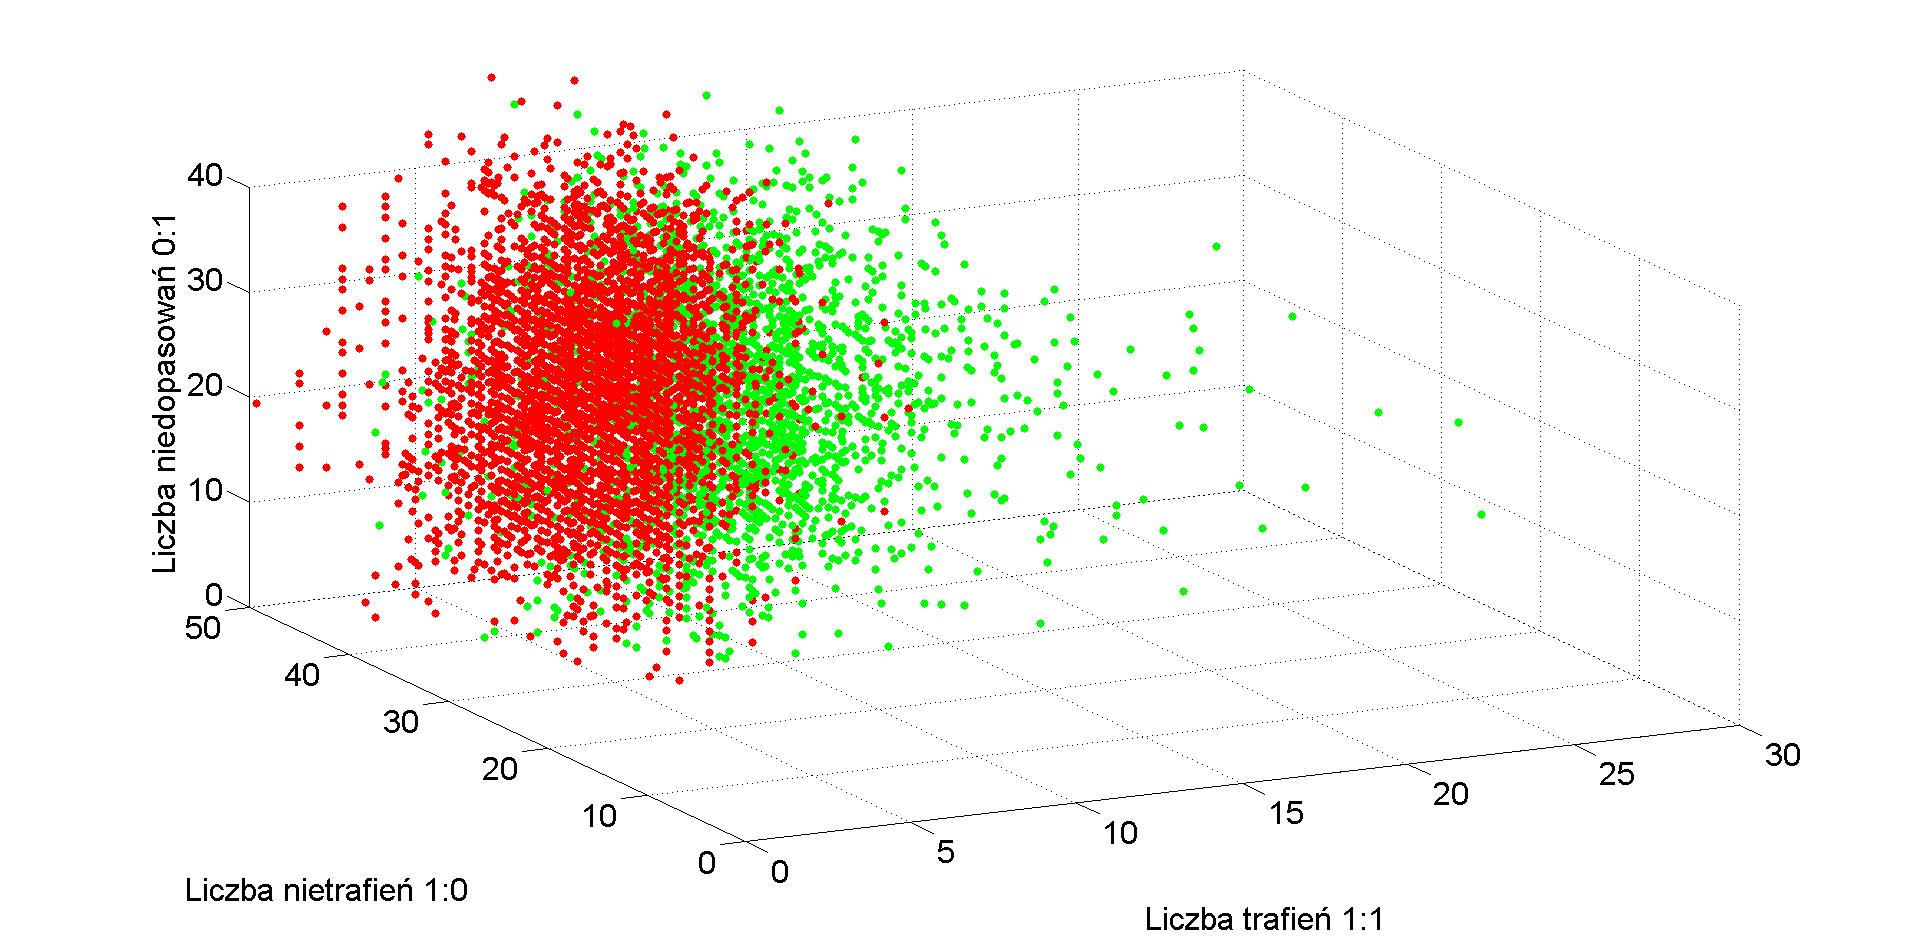
\includegraphics[angle=0,scale=0.27]{img/cloud.jpg}
		\caption{Rozkład punktów dopasowań dla porównań kodów odcisku}
		\label{img:cloud_all}
    \end{center}
\end{figure} 

\begin{figure}[!hbt]
    \begin{center}
		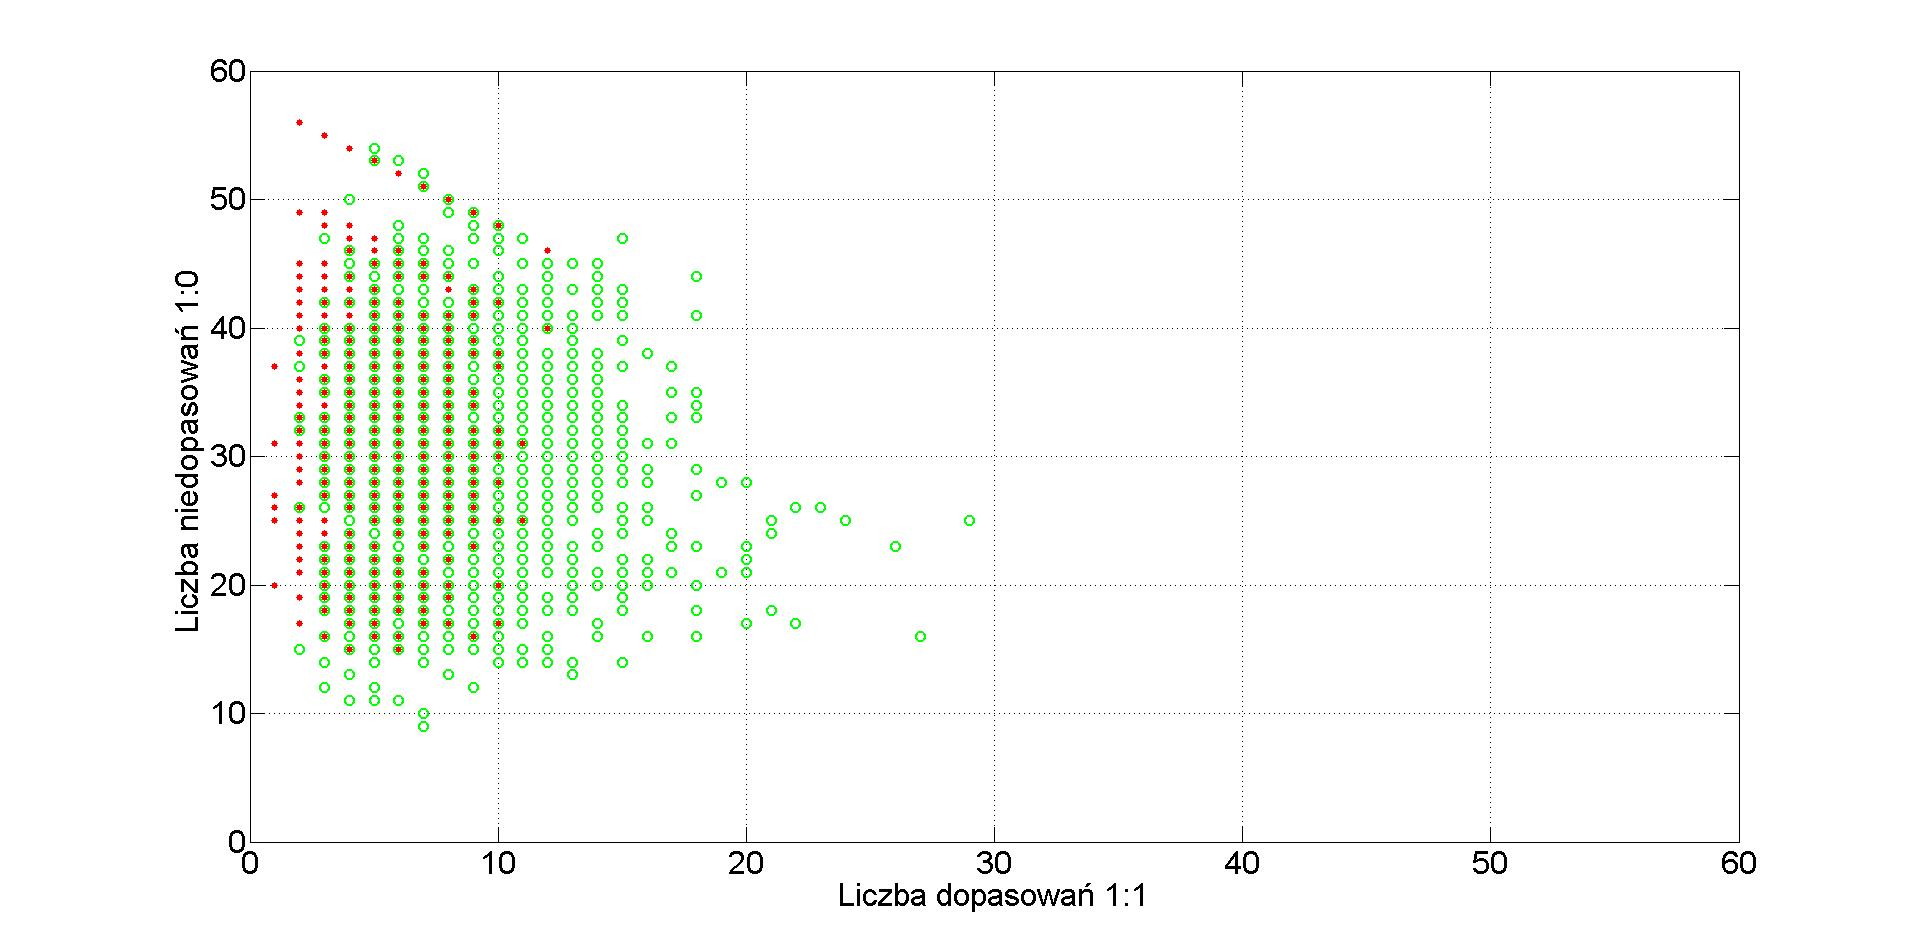
\includegraphics[angle=0,scale=0.27]{img/cloud_1.jpg}
		\caption{Rozkład punktów dopasowań dla porównań kodów odcisku na przestrzeni porównań (1:1) (1:0)}
		\label{img:cloud_1}
    \end{center}
\end{figure} 

\begin{figure}[!hbt]
    \begin{center}
		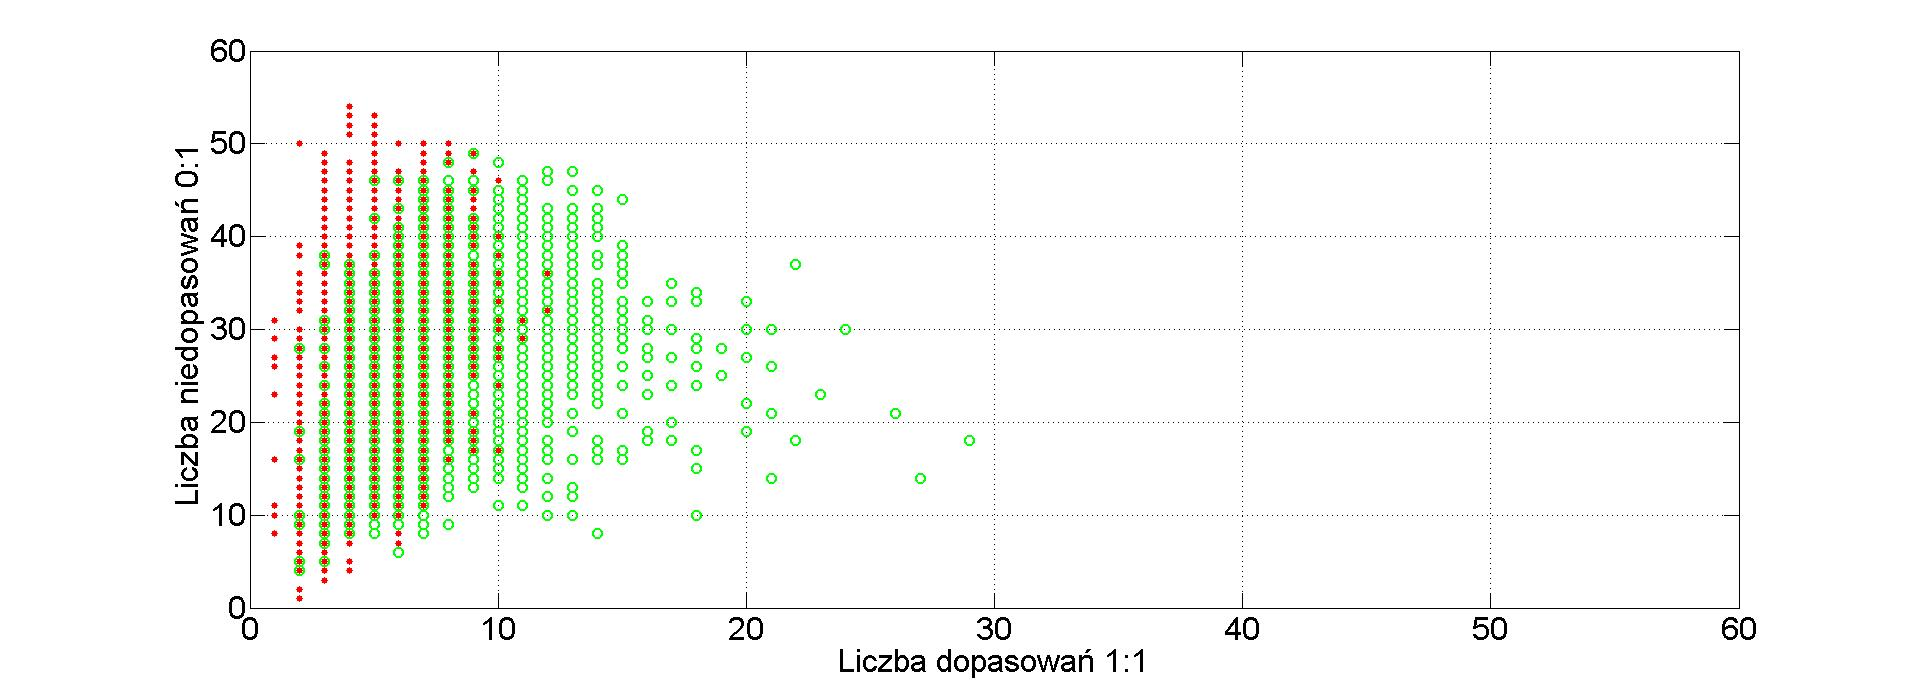
\includegraphics[angle=0,scale=0.27]{img/cloud_2.jpg}
		\caption{Rozkład punktów dopasowań dla porównań kodów odcisku na przestrzeni porównań (1:1) (0:1)}
		\label{img:cloud_2}
    \end{center}
\end{figure} 

\begin{figure}[!hbt]
    \begin{center}
		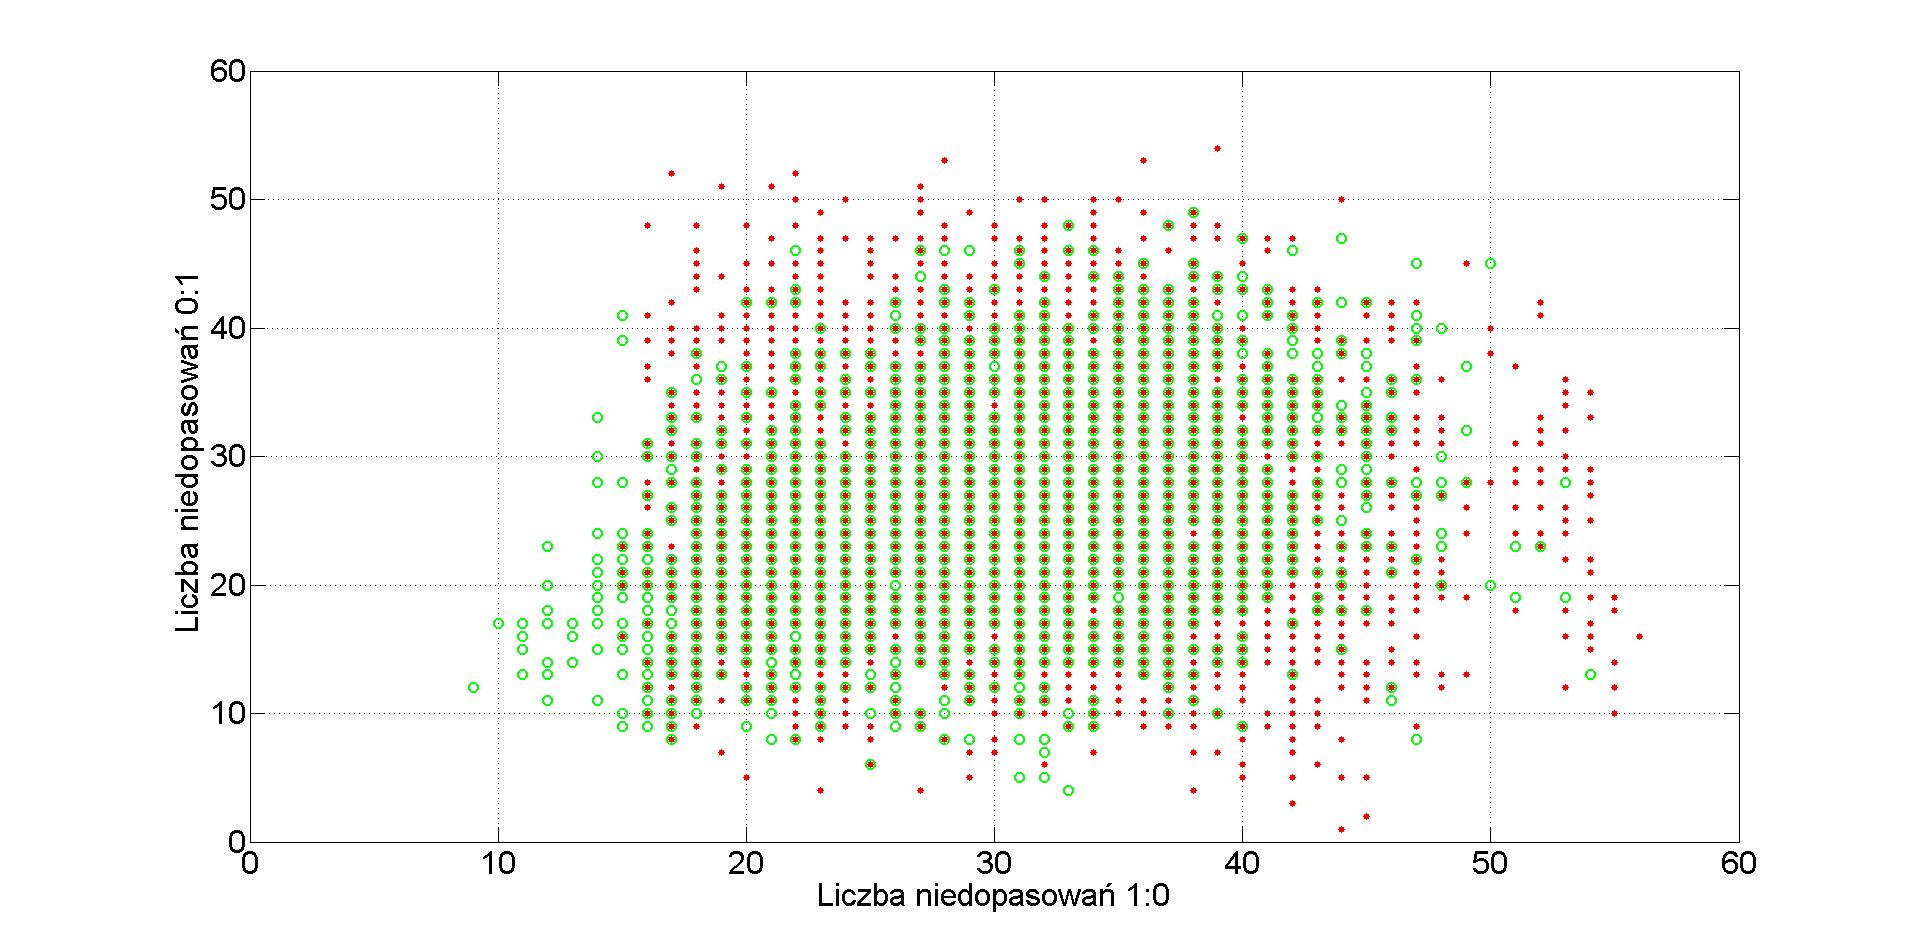
\includegraphics[angle=0,scale=0.27]{img/cloud_3.jpg}
		\caption{Rozkład punktów dopasowań dla porównań kodów odcisku na przestrzeni porównań (1:0) (0:1)}
		\label{img:cloud_3}
	\end{center}
\end{figure} 
\chapter {Różnica symetryczna jako sposób porównywania odcisków}

Większość obecnie stosowanych metod porównuje odciski poprzez szukanie podobieństw między nimi. Metody nie zastanawiają się nad wpływem ilości niepodobnych minucji. Celem tej pracy jest stwierdzenie czy istnieje możliwość porównywania odcisków badając jedynie ich niepodobieństwo. Sposób ten stara się odpowiedzieć na pytanie co jest lepsze 10 zgodnych minucji, które stanowią jedynie 33\% wszystkich minucji, czy wzorca, czy 4 zgodne minucje które stanowią 50\% minucji wzorca. W obecnie stosowanych standardach liczba cech wspólnych wymaganych przez prawo lub procedury kryminalistyczne do ustalenia tożsamości wynosi\footnote{dane zaczerpnięte ze strony http://pl.wikipedia.org/wiki/Linie\_papilarne}
\renewcommand*{\labelitemi}{\bullet}
\begin{itemize}
	\item 8-12 Niemcy
	\item 17 Francja
	\item 15 Polska
\end{itemize}
\vspace{.5cm}\par
A w przypadku minucji rzadziej występujących liczba ich może być nawet mniejsza. Natomiast nigdzie nie doszukano się maksymalnych liczb niezgodnych minucji. Jedyne dodatkowe ograniczenia wprowadzają same SDK'i. Przykładowo SDK $Neurotechnology$ w standardowej konfiguracji przyjmuje minimalną liczbę minucji jako 10. Nie jest to jednak, żadna arbitralnie wyznaczana przez prawo wartość, a jej wartość można ustalać według własnych preferencji. Powstało założenie, że liczba minucji niezgodnych powinna być większa dla porównań między różnymi odciskami. Metoda podobnie jak sprawdzanie podobieństwa wrażliwa jest na liczbę minucji w porównywanych odciskach. Dlatego warto uzyskaną liczbę niezgodność podzielić przez ilość minucji w odciskach. Nie stosuje się oddzielnych statystyk dla niezgodności porównań 1:0 i 0:1. Statystyki te to nic innego jak porównywania przedstawione w rozdziale 4. Istnieje liniowa zależność między porównaniami co prezentuje wzór \ref{eq:dependency}.

\begin{equation}
Q_s = \frac{C_{1-1}}{C_{pattern}}
\label{eq:Q_s}
\end{equation}

\begin{equation}
Q_{ns} = \frac{C_{1-0}}{C_{pattern}}
\label{eq:Q_ns}
\end{equation}

\begin{equation}
Q_s = 1 - Q_{ns} 
\label{eq:dependency}
\end{equation}

\begin{table}
\begin{tabular}{l l p{13cm}}
\bullet & Q_s &  Jakość kodu(procent zgodności) \\
\bullet & Q_{ns} & Jakość kodu(procent niezgodności)\\
\bullet & C_{1-1} & Ilość porównań 1:1 dla \\
\bullet & C_{1-0} & Ilość porównań 1:0 \\
\bullet & C_{pattern} & Ilość minucji we wzorcu\\
\end{tabular}
\end{table}

\section[Analiza statystyczna kodu][Analiza statystyczna kodu]{Analiza statystyczna kodu}
Zastosowane rozwiązanie wylicza jakość niedopasowania jako iloraz sumy ilości porównań 1:0 i 0:1 do sumy ilości minucji wzorca i rozpatrywanych minucji próbki. Rozwiązanie przedstawia wzór\ref{eq:Q_nss}

\begin{equation}
Q_nss = 1 - \frac{C_{1-1}}{(C_{pattern} + C_{sample})}
\label{eq:Q_nss}
\end{equation}

\begin{table}
\begin{tabular}{l l p{13cm}}
\bullet & Q_{nss} & Jakość kodu(procent niezgodności) dla różnicy symetrycznej\\
\bullet & C_{sample} & Ilość rozpatrywanych minucji w próbce\\
\end{tabular}
\end{table}

W odróżnieniu od poprzedniego jest liniowo niezależny od jakości kodu przedstawianych w rozdziale 4. Gdyby tak nie było zabieg taki nie miałby większego sensu. Podobnie jak w poprzednim rozdziale świadomie zastąpiono odległości Hamminga porównując jedynie charakterystyczne porównania. Zbędne tło (porównania 0:0) jest pomijane. Wyniki z komercyjnego oprogramowania przedstawiane są jako porównanie. Podobnie jak wcześniej SDK $Neurotechnology$ użyto jedynie do zdobycia liczby minucji zgodnych i niezgodnych. Liczba porównań jest taka sama jak w poprzednim rozdziale i przeprowadzona została na tej samej próbie odcisków.

\subsection{Rezultaty testów}
Kolorem czerwonym zaznaczono porównania między odciskami pochodzącymi od różnych palców, zielonym pochodzących od tych samych. Przedstawione wyniki również nie są wystarczajaco dobre, natomiast są nieco lepsze niż w przypadku porównywania podobieństwa. EER zmniejszył się i wynosi ok 17\%. Nie jest to wynik zadowalający ale warto zauważyć, że zmieniono jedynie sposób porównania a nie sam algorytm kodowania. Każda poprawa wyniku jest więc sukcesem. FAR dla ustalonego progu wynosi ok 13\% i w porównaniu do poprzedniej metody uległ niewielkiemu pogorszeniu( 2 punkty procentowe). FRR wynosi ok 18\% i uległo sporej poprawie względem poprzedniej metody (5 punktów procentowych). Błędy ZERO FAR i ZERO FRR dalej są na poziomie niedopuszczalnym i wynoszą ponad 95\%. Kolejnym ciekawym zjawiskiem jest zwężenie przedziałów w jakich znajdują się wykresy. Niestety zmiana ta dotyczy zarówno porównań różnych jak i tych samych odcisków. Przedstawiona symulacja dowodzi iż sposoby porównywania niezgodności lepiej sprawdza się dla porównywania odcisków pochodzących od jednego palca. Natomiast sposób porównywania zgodności lepiej sprawdza się dla porównywania odcisków pochodzących od różnych palców. Wynik jest zaskakujący gdyż działa inaczej niż wskazywałoby na to logiczne rozumowanie. 

\subsubsection{Teza 1}
Stwierdzanie podobieństwa jest skuteczniejsze poprzez porównywanie niepodobieństw.

\subsubsection{Teza 2}
Stwierdzanie niepodobieństwa jest skuteczniejsze poprzez porównywanie podobieństw.
\vspace{.5cm}\par

Plusem tej metody jest brak konieczności rozstrzygania wyniku dla porównań względem próbki i dla porównań względem wzorca. W poprzedniej metodzie właściwie otrzymywano dwa wskazania w zależności czy liczbę dopasowań podzielono przez liczbę minucji wzorca czy liczbę rozpatrywanych minucji próbki. W tej metodzie wyróżniono tylko jeden współczynnik. Możliwym wyjściem jest stosowanie hybrydy tych dwóch rozwiązań. Zastosować można to dla tych porównań które znajdują się blisko progu decyzyjnego. w takiej sytuacji należało by skorzystać z drugiego wskaźnika i w przypadku przeciwnego rezultatu, wybrać ten który znajduje się dalej od swego progu decyzyjnego. Być może taka hybryda łączyła by mocne strony obu sposobów porównań mogłoby to doprowadzić do kolejnego zmniejszenia błędów dopasowań odcisków. 

\begin{figure}[!htb]
    \begin{center}
		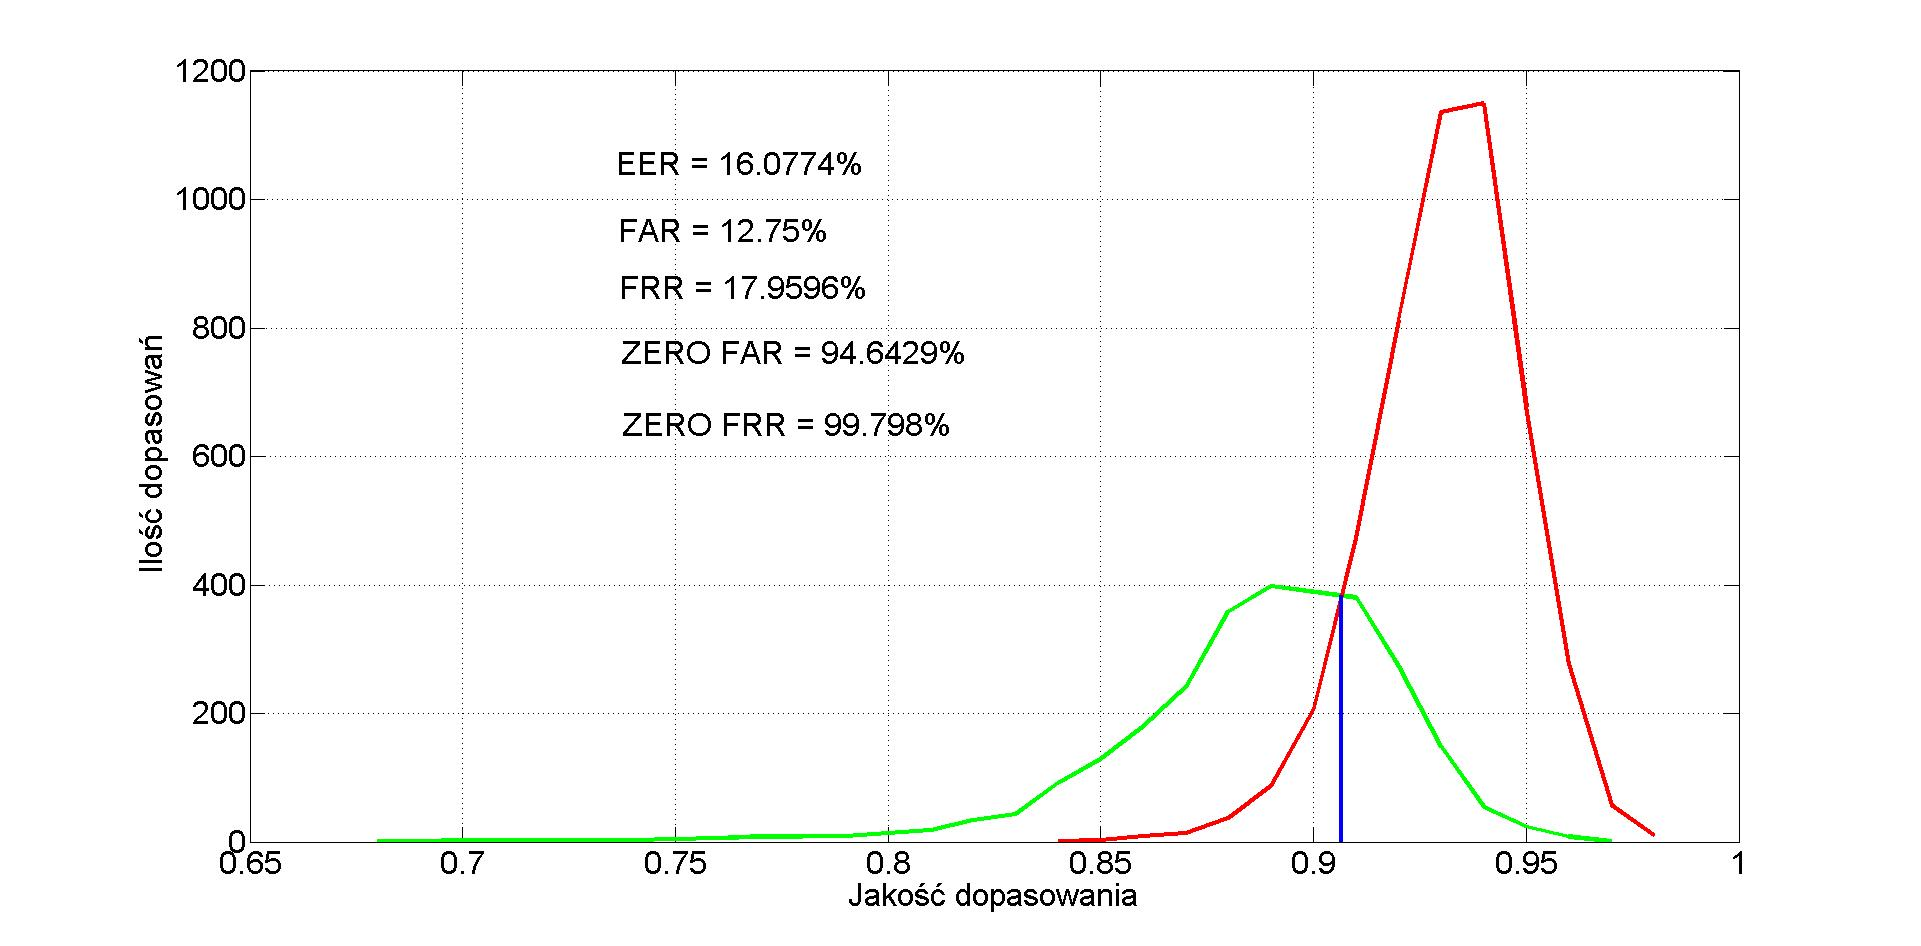
\includegraphics[angle=0,scale=0.27]{img/simetric_distance_code_line.jpg}
		\caption{Ilość niedopasowań w zależności od jakości niedopasowania do odcisków}
		\label{img:code_simetric_line}
    \end{center}
\end{figure} 
Niestety test ten dowodzi iż niezależnie od metody porównywania dla zaproponowanego algorytmu jest nieskuteczne jeśli porównujemy tylko jeden wskaźnik takiego porównania. Niezależnie czy porównujemy podobieństwo czy niepodobieństwo błąd EER jest niedopuszczalny i nie czyni tworzonej metody systemem biometrycznym. Celowo nie sprawdzam hybrydowego rozwiązania gdyż nawet polepszenie wyniku o kilka punktów procentowych nie jest rozwiązaniem. Jedyną drogą rozwiązania problemu jest wykorzystanie wszystkich danych tworzonych przez porównywanie i badanie rozkładu punktów porównań w przestrzeni trójwymiarowej. Metoda oraz jej wyniki opisana jest w rozdziale 6.
\vspace{.5cm}\par

Na wykresie \ref{img:ob_simetric_line} Przedstawiono tą samą metodę wykorzystując SDK $Neurotechnology$ jedynie do zdobycia liczby minucji pasujących i niepasujących. W zastosowaniu algorytmu kodującego, jak również dla listy minucji z SDK'a zaobserwowano poprawę wskaźnika EER i FRR wskaźnik FAR został bez zmian. Ponieważ zmiana zachowań współczynników jest powtarzalna dla podejścia kodowego i obiektowego, dlatego tezy 1 i 2 można uznać za prawdziwe. Plusem tej obserwacji jest to iż postawione tezy nie zależą od stosowanych algorytmów. Podobnie jak w porównywaniu podobieństwa dane zebrane z komercyjnego SDK mają lepsze wyniki od podejścia kodowego. Dowodzi to iż kodowa wersja algorytmu w połączeniu z tymi metodami porównywania odcisków nie jest wystarczająco dobra do poprawnej weryfikacji. 

\begin{figure}[!htb]
    \begin{center}
		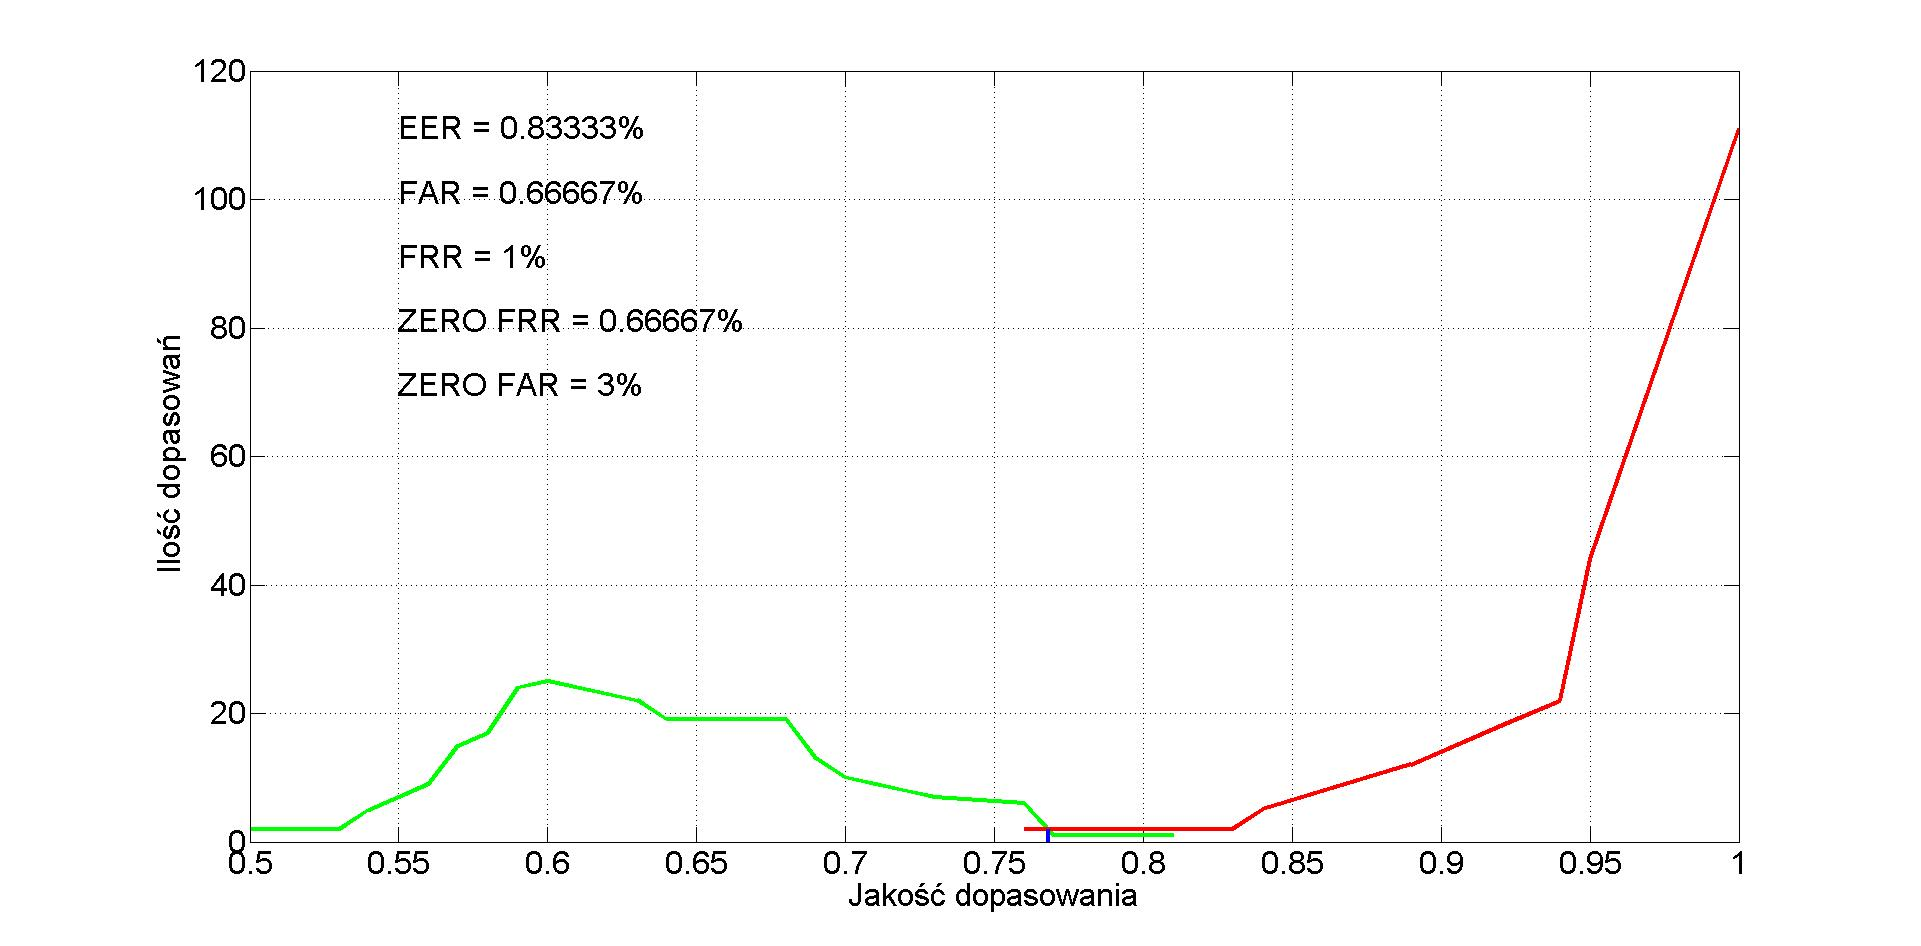
\includegraphics[angle=0,scale=0.27]{img/simetric_distance_ob_line.jpg}
		\caption{Ilość niedopasowań w zależności od jakości niedopasowania do odcisków}
		\label{img:ob_simetric_line}
    \end{center}
\end{figure} 
\chapter{Metoda 3D porównywania kodów}
Metoda opiera się na porównywaniu poprzez wykorzystanie wszystkich danych o porównaniu kodów. Decyzje o weryfikacji odcisku podejmowana jest poprzez analizę podobieństwa i niepodobieństwa jednocześnie. Do dyspozycji są 3 porównania, ale ponieważ rozkład punktów porównania 1:0 i porównania 0:1 jest prawie taki sam podjęto decyzję o pominięciu tego porównania w procesie weryfikacji. Podobnie jak w poprzednich rozdziałach sposób działania będzie porównywany z wynikami otrzymanymi od SDK $Neurotechnology$. Ten sposób porównania ma służyć nie tylko polepszeniu ogólnego wyniku algorytmu ale też i sposobu porównywania bazującego tylko na liczbie minucji dopasowanych i niedopasowanych. Niemożliwe jest jednak przedstawianie błędów w takiej samej konwencji jak w poprzednich rozdziałach. Wynika to z tego iż próg decyzyjny nie dobierany jest w taki sposób aby równoważyć błąd FAR i FRR, a poprzez tworzenie funkcji separującej zbiory punktów od siebie. Jest to o tyle kłopotliwe iż nie mam możliwości manipulowania progiem decyzyjnym tak samo jak w poprzednich rozdziałach.
Przedstawiane wyniki to wartości błędnych decyzji dopasowania i niedopasowania. Mimo iż rozpatrujemy rozkład punktów na płaszczyźnie metoda została nazwana porównaniem 3D, gdyż do weryfikacji używa trzech rodzajów porównań.
\section [Opis metody][Opis metody]{Opis metody}
Testy metody wykonano na tej samej grupie porównań co testy opierające się na badaniu podobieństwa i nie podobieństwa. Zbiór ten podzielono na dwie części, część uczącą i część testującą. Część ucząca odpowiada za utworzenie funkcji separującej oba zbiory porównań, część testująca wykorzystana jest do testów poprawnej weryfikacji dla utworzonej funkcji separującej. Testy prowadzone są w trzech wariantach
\renewcommand*{\labelitemi}{\bullet}
\begin{itemize}
	\item Rozkład porównań 1:1 do sumy porównań 1:0 i 0:1
	\item Rozkład porównań 1:1 do 1:0
	\item Rozkład porównań 1:1 do 0:1
\end{itemize}
\vspace{.5cm}\par
Dla potrzeb tej pracy wybrano metodę Maszyny wektorów nośnych\footnote{SVM z ang. support vector machine - klasyfikator, którego nauka ma na celu wyznaczenie hiperpłaszczyzny rozdzielającej z maksymalnym marginesem przykłady należące do dwóch klas.} oraz skorzystano z gotowych implementacji tej metody w środowisku MATLAB. W trakcie testów klasyfikator tworzy hiperpłaszczyzną separująca zbiory punktów, a następnie testuje wyniki dla zbioru testującego. Dopuszczalne są przypadki nie w pełni separowane. Oznacza to, że metoda ta może wnosić błąd już dla swojego zbioru uczącego. Kształt hiperpłaszczyzny zależy nie tylko od rozkładu punktów ale też od używanego jądra. Testy przeprowadzono dla czterech wariantów
\begin{itemize}
\item Liniowe
\item Kwadratowe
\item Wielomianowe
\item Normalne(Gaussowskie)
\end{itemize}
\vspace{.5cm}\par
Zbiór uczący oraz zbiór porównań jest równo liczny choć liczba punktów uczących oraz liczba punktów na których przeprowadzane są testy może się różnić. Wynika to z tego iż rozkład liczby punktów porównań nie jest unikalny i powtarza się dla różnych porównań odcisków. Istnieją różne odciski o dokładnie o takiej samie liczbie minucji zgodnych i niezgodnych.
\section [Wyniki][Wyniki]{Wyniki}
\begin{figure}[!htb]
    \begin{center}
		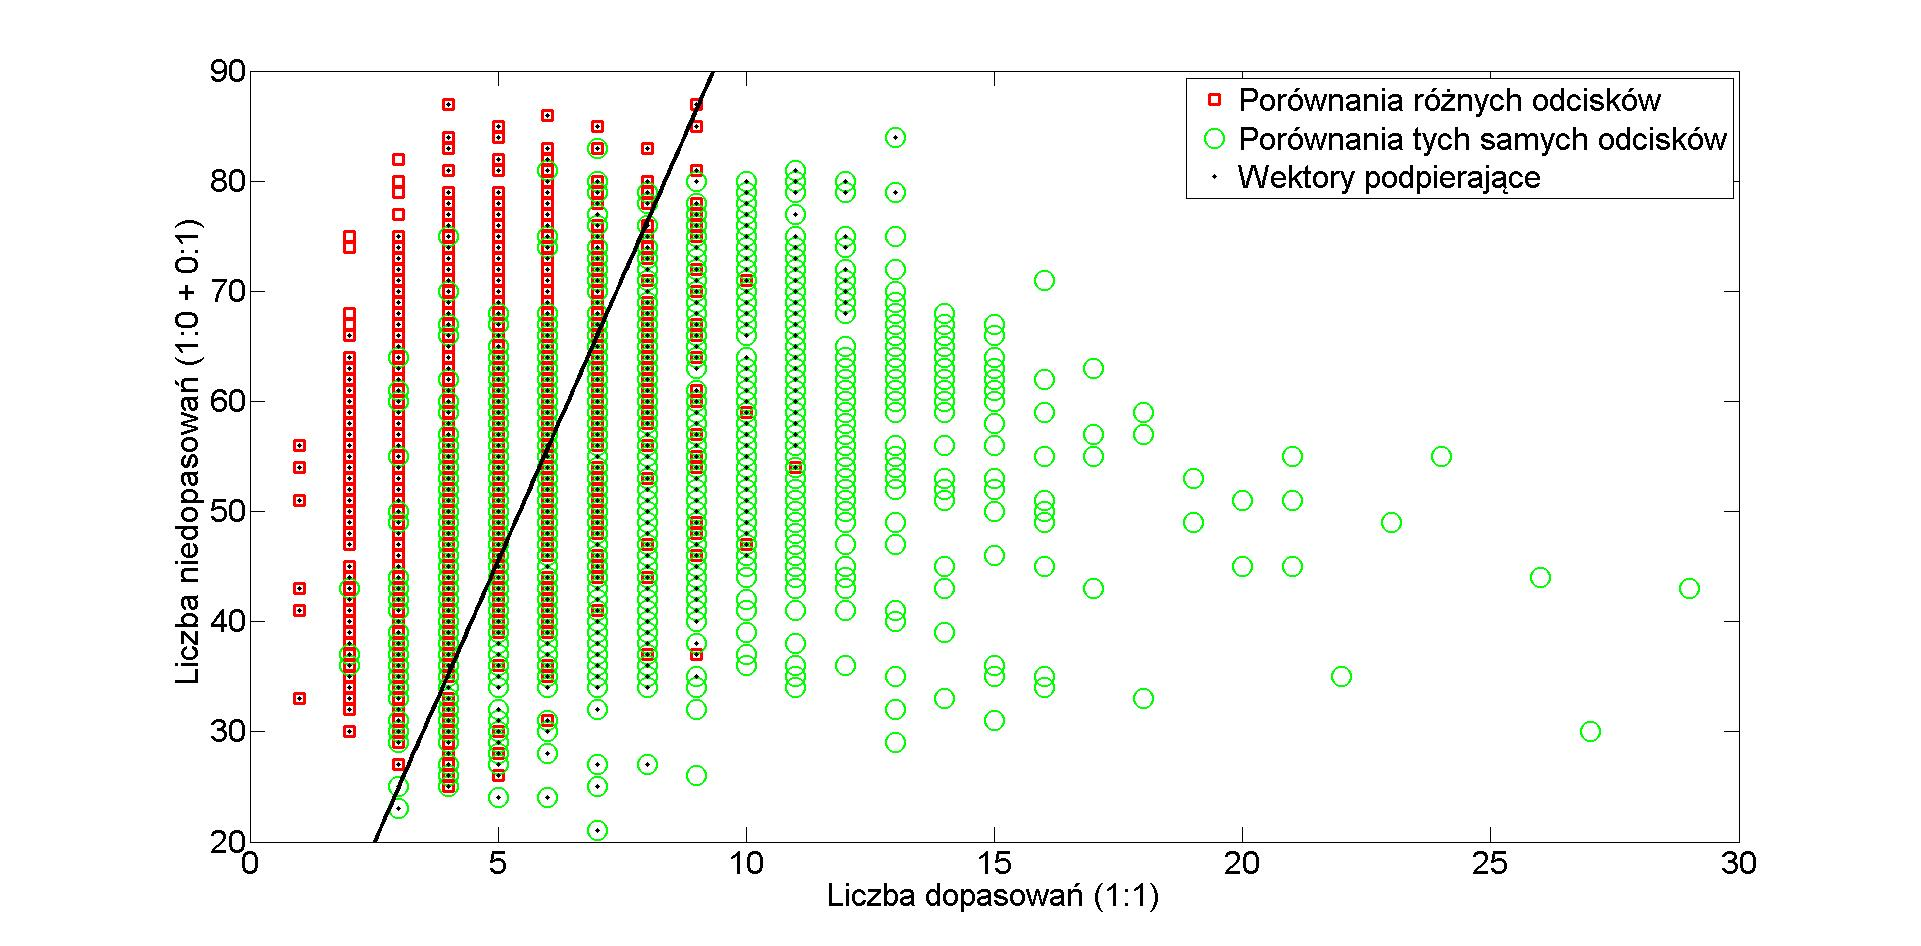
\includegraphics[angle=0,scale=0.27]{img/SVM_linear_code_1.jpg}
		\caption{Separacja punktów dla jądra liniowego}
		\label{img:SVM_linear_code_1}
    \end{center}
\end{figure} 

Wykres \ref{img:SVM_linear_code_1} przedstawia liniową separacje punktów. Konsekwentnie zielonym kolorem zaznaczone są porównania między odciskami pochodzącymi od tego samego palca, czerwonym porównania między odciskami pochodzącymi od różnych palców. Doskonale widać iż nie możliwe jest liniowe separowanie punktów. Metoda już dla zbioru testowego wniesie pewien błąd. Nie jest to jednak ogromny problem. Możliwe jest bowiem stworzenie kilku równań prostych które w stu procentach rozdzielą oba zbiory. Niestety nie wpływa to na skuteczność metody, zbiór uczący powinien być w miarę uniwersalny, a funkcja powinna tylko uogólniać zachowanie punktów na płaszczyźnie. 

    \begin{table}[!htb]
    \begin{tabular}{p{3cm}|r||c|c|c|}
	\cline{2-5}
    & Wariant & \multicolumn{3}{|c|}{1:1 do 1:0 + 0:1}\\ \cline{2-5} 
    & Zbiór testujący & ERRORS  & FRR & FAR\\ \hline
	\multicolumn{2}{|l||}{Rodzaj jądra} &  \multicolumn{3}{|c|}{}\\
	\hline\hline
    \multicolumn{2}{|l||}{Liniowe} & 28.6722\% & 26.6393\% & 31.405\%\\ \hline
    \multicolumn{2}{|l||}{Kwadratowe} & 28.6722\% & 25.6148\% & 32.7824\%\\ \hline
    \multicolumn{2}{|l||}{Wielomianowe st. 3} & 28.9072\% & 29.3033\% & 28.3747\%\\ \hline
    \multicolumn{2}{|l||}{Wielomianowe st. 7} & 31.2573\% & 29.3033\% & 33.8843\%\\ \hline
    \multicolumn{2}{|l||}{Wielomianowe st. 12} & 29.3772\% & 32.7869\% & 24.7934\%\\ \hline
    \multicolumn{2}{|l||}{Normalne(Gaussowskie)} & 28.6722\% & 24.7951\% & 33.8843\%\\ \hline
    \end{tabular}
	\caption{Wyniki testów algorytmu kodowego metoda 3D porównywania kodów}
	\label{tab:3D_sum}
    \end{table}
    
    \begin{table}[!htb]
    \begin{tabular}{p{3cm}|r||c|c|c|}
	\cline{2-5}
    & Wariant & \multicolumn{3}{|c|}{1:1 do 1:0} \\ \cline{2-5} 
    & Zbiór testujący & ERRORS  & FRR & FAR\\ \hline
	\multicolumn{2}{|l||}{Rodzaj jądra} &  \multicolumn{3}{|c|}{}\\
	\hline\hline
    \multicolumn{2}{|l||}{Liniowe} & 29.6703\% & 13.6232\% & 57.2139\%\\ \hline
    \multicolumn{2}{|l||}{Kwadratowe} & 29.8535\% & 12.4638\% & 59.7015\%\\ \hline
    \multicolumn{2}{|l||}{Wielomianowe st. 3} & 29.3040\% & 7.8261\% & 66.1692\%\\ \hline
    \multicolumn{2}{|l||}{Wielomianowe st. 7} & 30.2198\% & 8.9855\% & 66.6667\%\\ \hline
    \multicolumn{2}{|l||}{Wielomianowe st. 12} & 36.8132\% & 35.3623\% & 39.3035\%\\ \hline
    \multicolumn{2}{|l||}{Normalne(Gaussowskie)} & 31.1355\% & 3.7681\% & 78.1095\%\\ \hline
    \end{tabular}
	\caption{Wyniki testów algorytmu kodowego metoda 3D porównywania kodów}
	\label{tab:3D_pattern}
    \end{table}
    
    \begin{table}[!htb]
    \begin{tabular}{p{3cm}|r||c|c|c|}
	\cline{2-5}
    & Wariant & \multicolumn{3}{|c|}{1:1 do 0:1} \\ \cline{2-5} 
    & Zbiór testujący & ERRORS  & FRR & FAR\\ \hline
	\multicolumn{2}{|l||}{Rodzaj jądra} &  \multicolumn{3}{|c|}{}\\
	\hline\hline
    \multicolumn{2}{|l||}{Liniowe} & 31.2024\% & 30.2778\% & 32.3232\% \\ \hline
    \multicolumn{2}{|l||}{Kwadratowe} & 30.5936\% & 31.6667\% & 29.2929\%\\ \hline
    \multicolumn{2}{|l||}{Wielomianowe st. 3} & 31.3546\% & 29.7222\% & 33.3333\%\\ \hline
    \multicolumn{2}{|l||}{Wielomianowe st. 7} & 34.2466\% & 43.0556\% & 23.5690\%\\ \hline
    \multicolumn{2}{|l||}{Wielomianowe st. 12} & 32.5723\% & 36.3889\% & 27.9461\%\\ \hline
    \multicolumn{2}{|l||}{Normalne(Gaussowskie)} & 31.2024\% & 29.7222\% & 32.9966\%\\ \hline
    \end{tabular}
	\caption{Wyniki testów algorytmu kodowego metoda 3D porównywania kodów}
	\label{tab:3D_sample}	
    \end{table}
    
   \begin{figure}[!htb]
    \begin{center}
		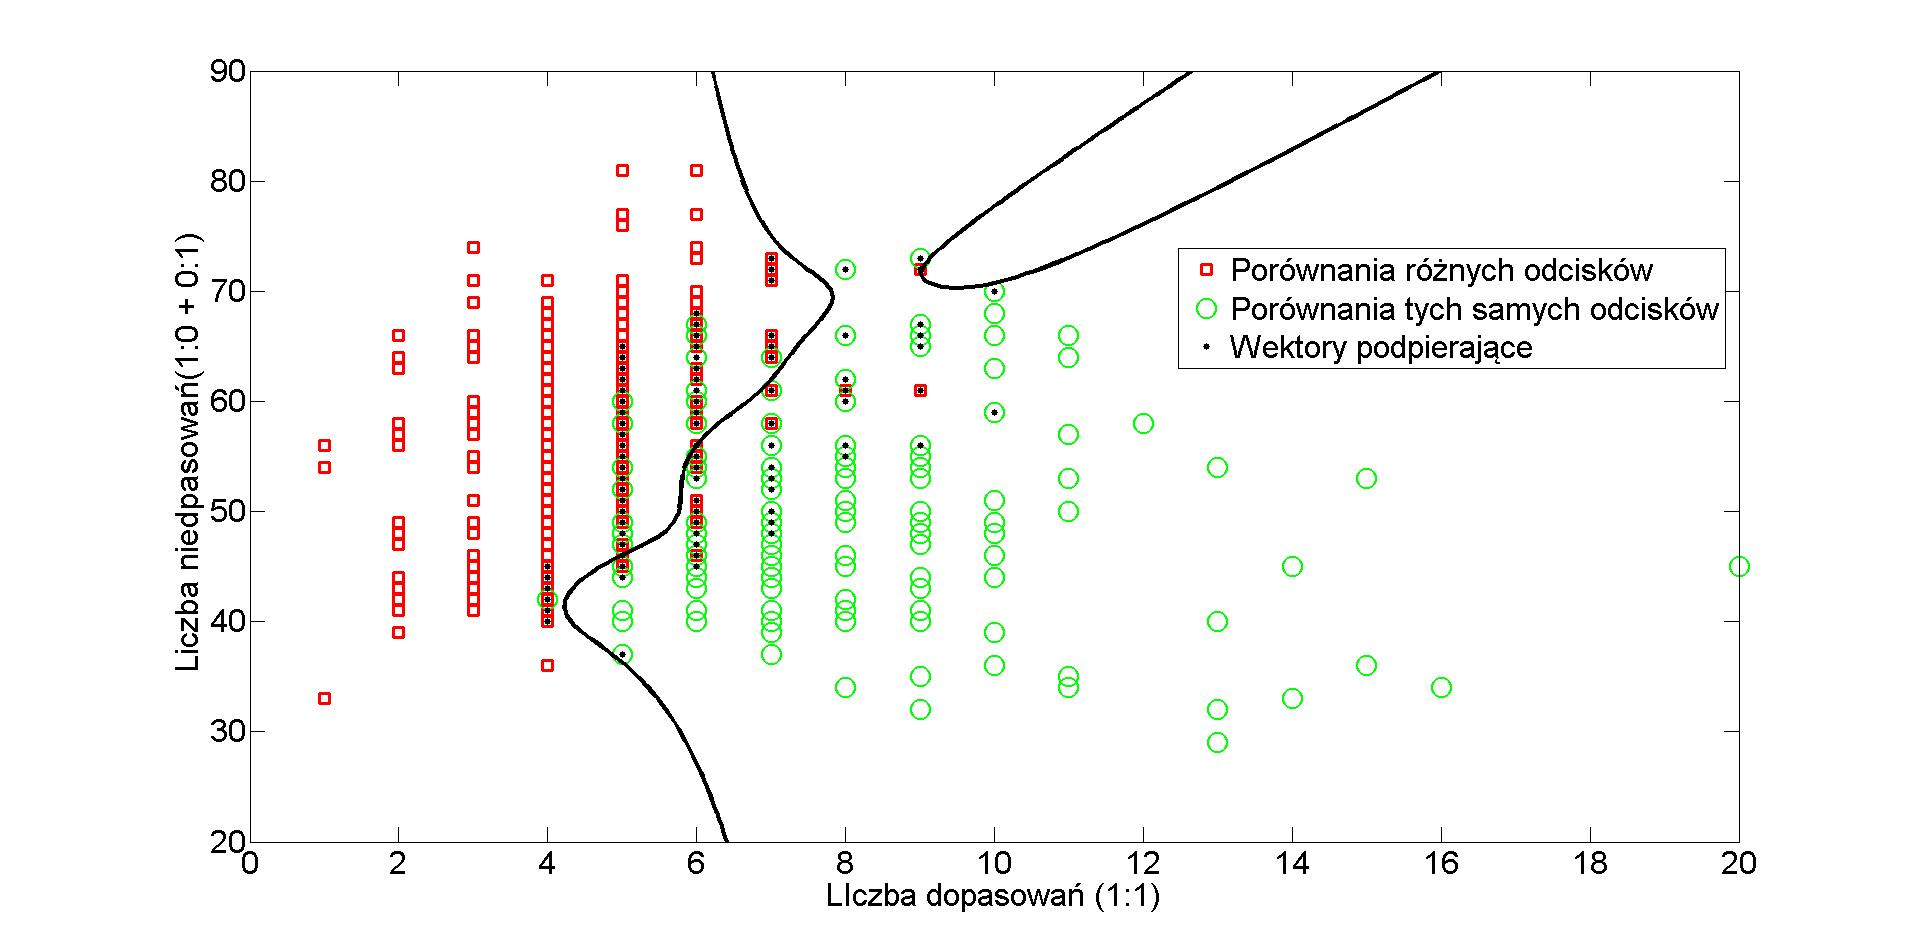
\includegraphics[angle=0,scale=0.27]{img/SVM_polynominal_code_1.jpg}
		\caption{Separacja punktów dla jądra wielomianowego stopnia 7}
		\label{img:SVM_polynominal_code_1}
    \end{center}
    \end{figure}
    
    \begin{figure}[!htb]
    \begin{center}
		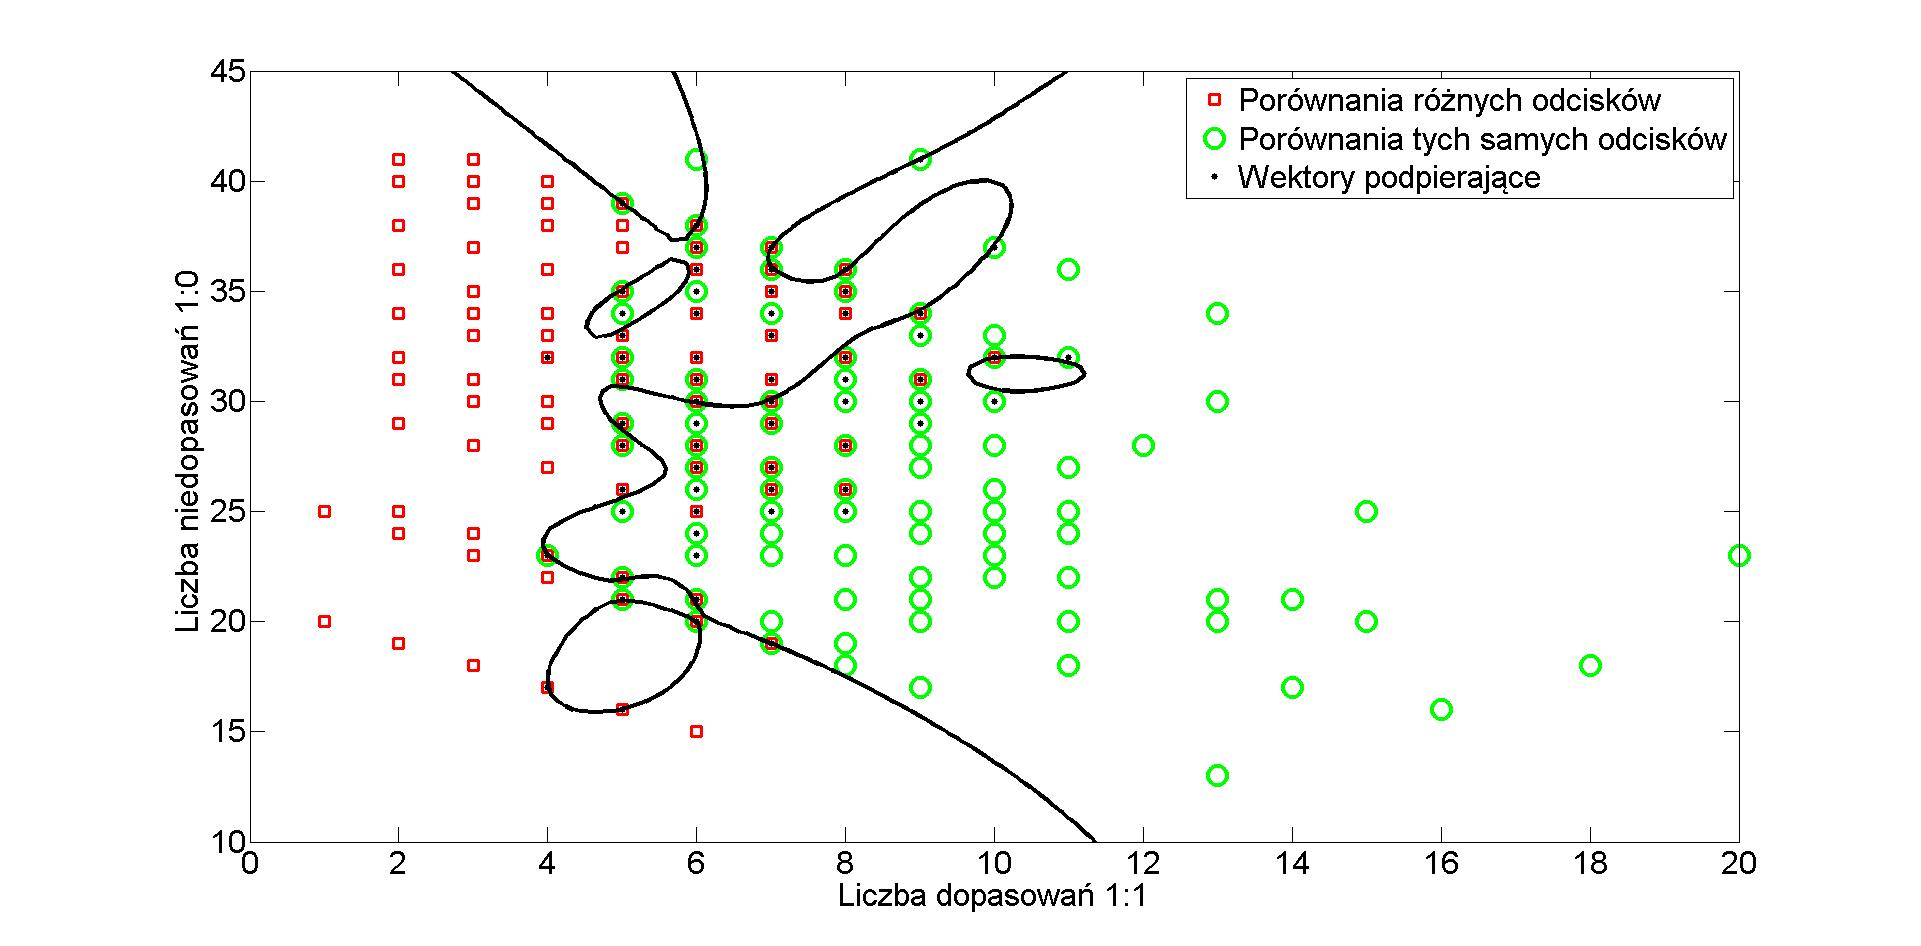
\includegraphics[angle=0,scale=0.27]{img/bad_st_12.jpg}
		\caption{Zły wpływ zbyt dużego stopnia jądra wielomianowego(12)}
		\label{img:best_SVM}
    \end{center}
    \end{figure} 
    
    \begin{figure}
    \begin{center}
		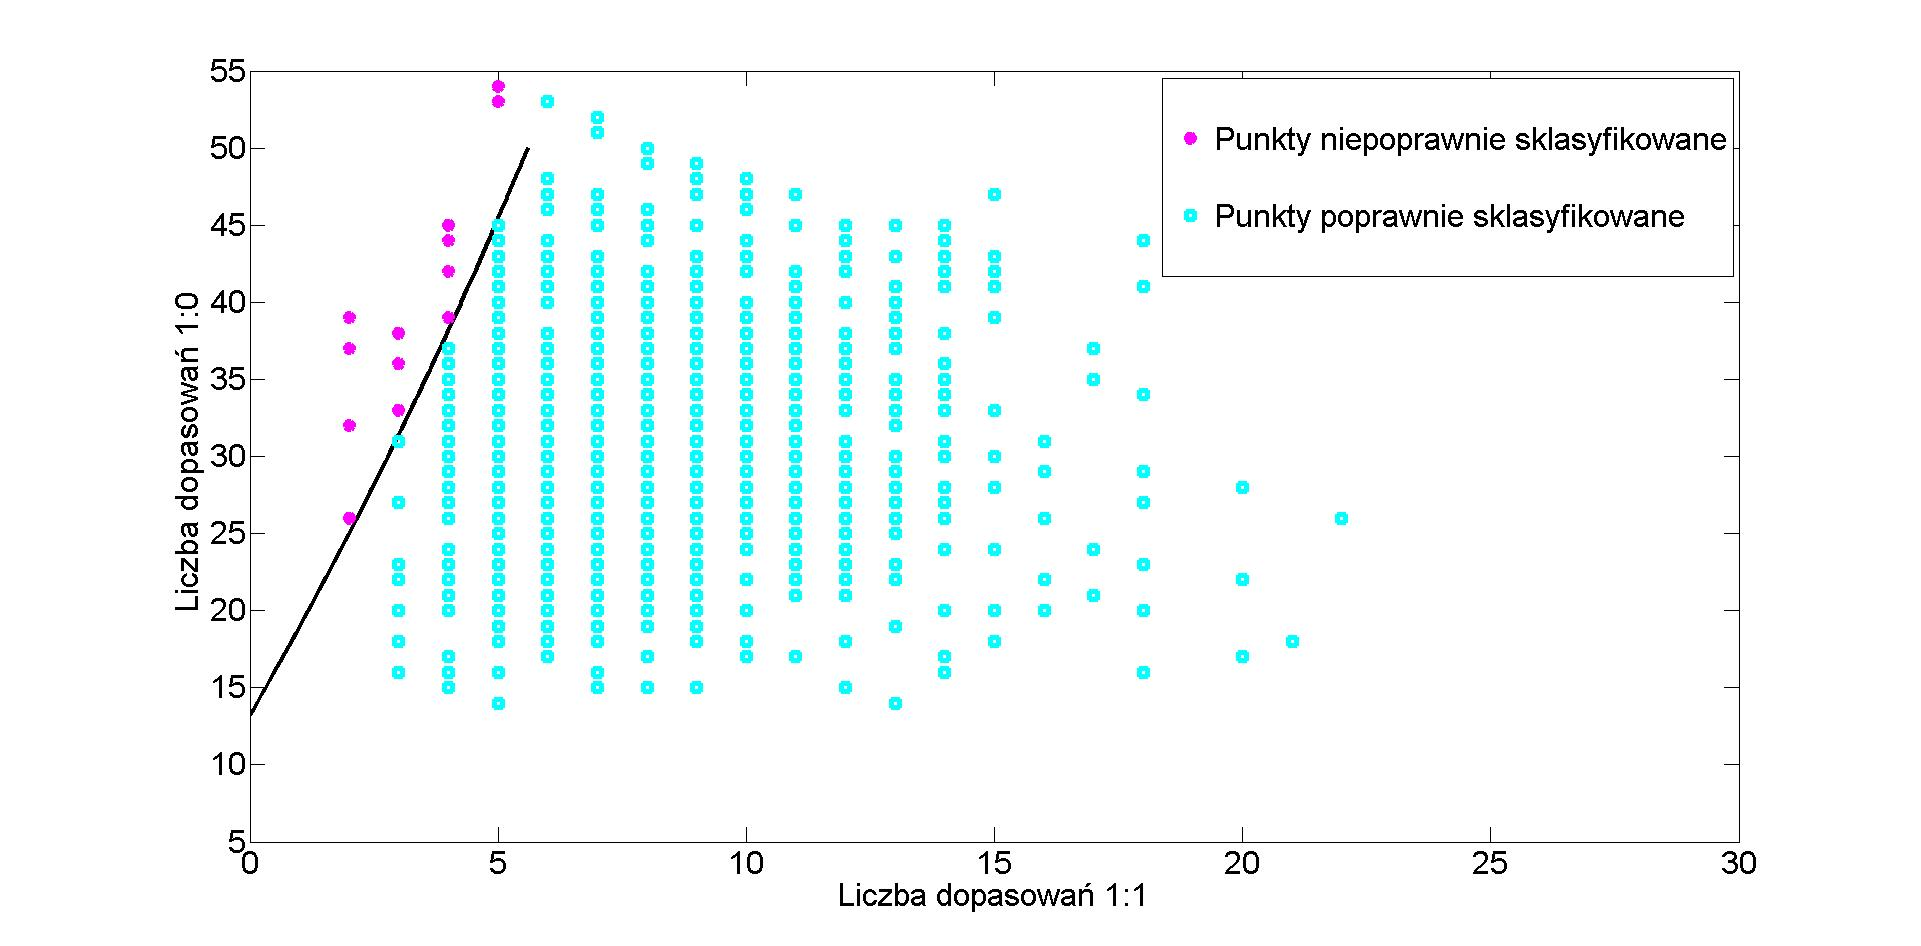
\includegraphics[angle=0,scale=0.27]{img/3D_best_score.jpg}
		\caption{Przykład klasyfikacji punktów algorytmu kodującego dla wariantu 1:1 do 1:0 jądro gaussowskie}
		\label{img:bad_SVM}
    \end{center}
    \end{figure} 
    
Tabele \ref{tab:3D_sum}, \ref{tab:3D_pattern}, \ref{tab:3D_sample} przedstawiają wyniki dla algorytmu kodującego. Widać, że pierwotne przypuszczenia rokujące poprawę jakości dopasowania były błędne. wyniki porównań znacznie się pogorszyły. Może to wynikać z niemożności znalezienia krzywej która w pełni separuje grupy punktów. Dodatkowo żaden z wariantów porównywania nie wyróżnia się na tle innych. Ilość błędnych decyzji jest podobna dla wszystkich wariantów i waha się od 28\% do 35\%. Jedyną wyraźną poprawę widać dla wskaźnika FRR dla wariantu porównań 1:1 do 1:0, gdzie dla jądra gaussowskiego wskaźnik ten wynosi ok 3\% , gdzie dla poprzednich metod wahał się od 17\% do 23\%. Niestety FAR dla tej metody wynosi ponad 78\% co oznacza iż skuteczniejszy byłby tu klasyfikator losowy. Poprawę wskaźnika FRR można motywować tym iż klasyfikator SVM uczył się tylko na wynikach wzorca, gdyż oba porównania 1:1 i 1:0 dotyczą minucji wzorca. Niestety analogiczna sytuacja dla próbki gdzie klasyfikator uczył się na porównaniach 1:1 i 0:1 nie wykazała poprawy dla wskaźnika FAR. Gdyby tak się stało sensowne było by uczenie się na klasyfikatora SVM nie w przestrzenie dwu a trzy-wymiarowej. Dodatkowo większe skomplikowanie funkcji separującej nie przyczynia się do wzrostu tylko do spadku jakości porównania. Ponieważ nie do się idealnie rozsmarować punktów najlepiej spisują się metody o liniowym kształcie hiperprzestrzeni metody SVM. Zbyt zawiła funkcja prowadzi do bezsensownych rozgraniczeń takich ja pokazanych na rysunku \ref{img:bad_SVM}.

\begin{table}[!htb]
    \begin{tabular}{p{3cm}|r||c|c|c|}
	\cline{2-5}
    & Wariant & \multicolumn{3}{|c|}{1:1 do 1:0 + 0:1}\\ \cline{2-5} 
    & Zbiór testujący & ERRORS  & FRR & FAR\\ \hline
	\multicolumn{2}{|l||}{Rodzaj jądra} &  \multicolumn{3}{|c|}{}\\
	\hline\hline
    \multicolumn{2}{|l||}{Liniowe} & 0.4975\% & 0.0\% & 1.3889\%\\ \hline
    \multicolumn{2}{|l||}{Kwadratowe} & 0.4975\% & 0.0\% & 1.3889\%\\ \hline
    \multicolumn{2}{|l||}{Wielomianowe st. 3} &0.4975\% & 0\% & 1.3889\%\\ \hline
    \multicolumn{2}{|l||}{Wielomianowe st. 7} & 0.9950\% & 0.7752\% & 1.3889\%\\ \hline
    \multicolumn{2}{|l||}{Wielomianowe st. 12} & 0.9950\% & 0.7752\% & 1.3889\%\\ \hline
    \multicolumn{2}{|l||}{Normalne(Gaussowskie)} & 0.4975\% & 0\% & 1.3889\%\\ \hline
    \end{tabular}
	\caption{Wyniki testów algorytmu kodowego metoda 3D porównywania kodów}
	\label{tab:3D_sum_2}
    \end{table}
    
    \begin{table}[!htb]
    \begin{tabular}{p{3cm}|r||c|c|c|}
	\cline{2-5}
    & Wariant & \multicolumn{3}{|c|}{1:1 do 1:0} \\ \cline{2-5} 
    & Zbiór testujący & ERRORS  & FRR & FAR\\ \hline
	\multicolumn{2}{|l||}{Rodzaj jądra} &  \multicolumn{3}{|c|}{}\\
	\hline\hline
    \multicolumn{2}{|l||}{Liniowe} & 2.5641\% & 2.0\% & 5.8824\%\\ \hline
    \multicolumn{2}{|l||}{Kwadratowe} & 1.7094\% & 1.0\% & 5.8824\%\\ \hline
    \multicolumn{2}{|l||}{Wielomianowe st. 3} & 1.7094\% & 1.0\% & 5.8824\%\%\\ \hline
    \multicolumn{2}{|l||}{Wielomianowe st. 7} & 2.5641\% & 2.0\% & 5.8824\%\\ \hline
    \multicolumn{2}{|l||}{Wielomianowe st. 12} & 6.8376\% & 7.0\% & 5.8824\%\\ \hline
    \multicolumn{2}{|l||}{Normalne(Gaussowskie)} & 11.1111\% & 0\% & 76.4706\%\\ \hline
    \end{tabular}
	\caption{Wyniki testów algorytmu kodowego metoda 3D porównywania kodów}
	\label{tab:3D_pattern}
    \end{table}
    
    \begin{table}[!htb]
    \begin{tabular}{p{3cm}|r||c|c|c|}
	\cline{2-5}
    & Wariant & \multicolumn{3}{|c|}{1:1 do 0:1} \\ \cline{2-5} 
    & Zbiór testujący & ERRORS  & FRR & FAR\\ \hline
	\multicolumn{2}{|l||}{Rodzaj jądra} &  \multicolumn{3}{|c|}{}\\
	\hline\hline
    \multicolumn{2}{|l||}{Liniowe} & 1.0638\% & 0.9091\% & 1.2821\% \\ \hline
    \multicolumn{2}{|l||}{Kwadratowe} & 0.5319\% & 0.0\% & 1.2821\%\\ \hline
    \multicolumn{2}{|l||}{Wielomianowe st. 3} & 0.5319\% & 0.0\% & 1.2821\%\\ \hline
    \multicolumn{2}{|l||}{Wielomianowe st. 7} & 1.0638\% & 0.9091\% & 1.2821\%\\ \hline
    \multicolumn{2}{|l||}{Wielomianowe st. 12} & 1.5957\% & 1.8182\% & 1.2821\%\\ \hline
    \multicolumn{2}{|l||}{Normalne(Gaussowskie)} & 0.5319\% & 0.0\% & 1.2821\%\\ \hline
    \end{tabular}
	\caption{Wyniki testów algorytmu kodowego metoda 3D porównywania kodów}
	\label{tab:3D_sample}	
    \end{table}
    
    Dla SDK $Neurotechnology$ wyniki generalnie uległy poprawie wahając się pierwotnie w granicach 0.8\% - 1.5\% dla porównywania oddzielnie podobieństwa i niepodobieństwa do najlepszych wyników ok 0.5\% dla porównywania 3D. Dla SDK najkorzystniejszym wariantem okazał się wariant uwzględniający porównania 1:1 do sumy 1:0 i 0:1. Przyczyną poprawy jest możliwość znalezienia funkcji "niemalże" separujących grupy punktów. Oznacza to, że sposób porównywania podobieństwa i niepodobieństwa jednocześnie podnosi skuteczność porównań. warunkiem koniecznym takiego zachowania jest możliwość separowania punktów porównań. W przeciwnym wypadku metoda prowadzi do pogarszania wyników.
    
\section[Wnioski][Wnioski]{Wnioski}

Metoda 3D porównywania kodów jest metodą której skuteczność jest ściśle uzależniona od rozkładu punktów  na płaszczyźnie i możliwości ich oddzielenia od siebie. W przypadku punktów których nie można odseparować metoda jedynie pogorszy uzyskiwane wyniki w stosunku do porównań tylko jednej cechy. Nie wskazane jest używanie zbyt zawiłych funkcji separujących. Klasyfikator powinien jedynie określać przybliżony rozkład punktów funkcje złożone powodują uczenie się na podstawie pojedynczych punktów, które nie mają odzwierciedlenia do całości zbioru porównań odcisków. Metoda nie gwarantuje 100\% skuteczności porównywania odcisków, ale istnieją takie konfiguracje metody gdzie pojedyncze współczynniki są pozbawione błędu(np FRR dla jadra liniowego wariantu porównań 1:1 do sumy 1:0 i 0:1 dla SDK $Neurotechnology$). Nie należy się jednak sugerować zbytnio otrzymanymi wynikami, twierdząc że powstała metoda bezbłędnie klasyfikująca odciski. Wszystko zależy od zbiory uczącego i zbioru testującego. 
Jednak opisana tu metoda dla SDK $Neurotechnology$ jest najlepszą z przedstawianych metod. 
 
    
\chapter{Ulepszenia}

W poprzednich rozdziałach przedstawiono wyniki algorytmu kodującego. Ponieważ nie są one zadowalające pomyślano nad sposobom poprawy algorytmu. Wadliwe działanie można usprawiedliwiać zbyt trudnym dopasowaniem kodów, ponieważ nie uwzględniano sąsiednich kratek kodowych. Podjęto więc decyzję o zmianie algorytmu w taki sposób aby porównywać nie tylko bezpośrednio odpowiadające kratki kodu, ale również ich sąsiadów. Tak więc dopasowanie jest nie tylko gdy zgodne są wszystkie współrzędne kodu x, y i kąt, ale również dopasowanie gdzie dowolna ze współrzędnych jest przesunięta o 1 kratkę kodową w górę lub w dól. Rozwiązanie sprzyja dopasowaniu kodów i powinno w jakiś sposób rekompensować nieliniowe przekształcenia opuszka palca. 
\begin{figure}[!htb]
    \begin{center}
		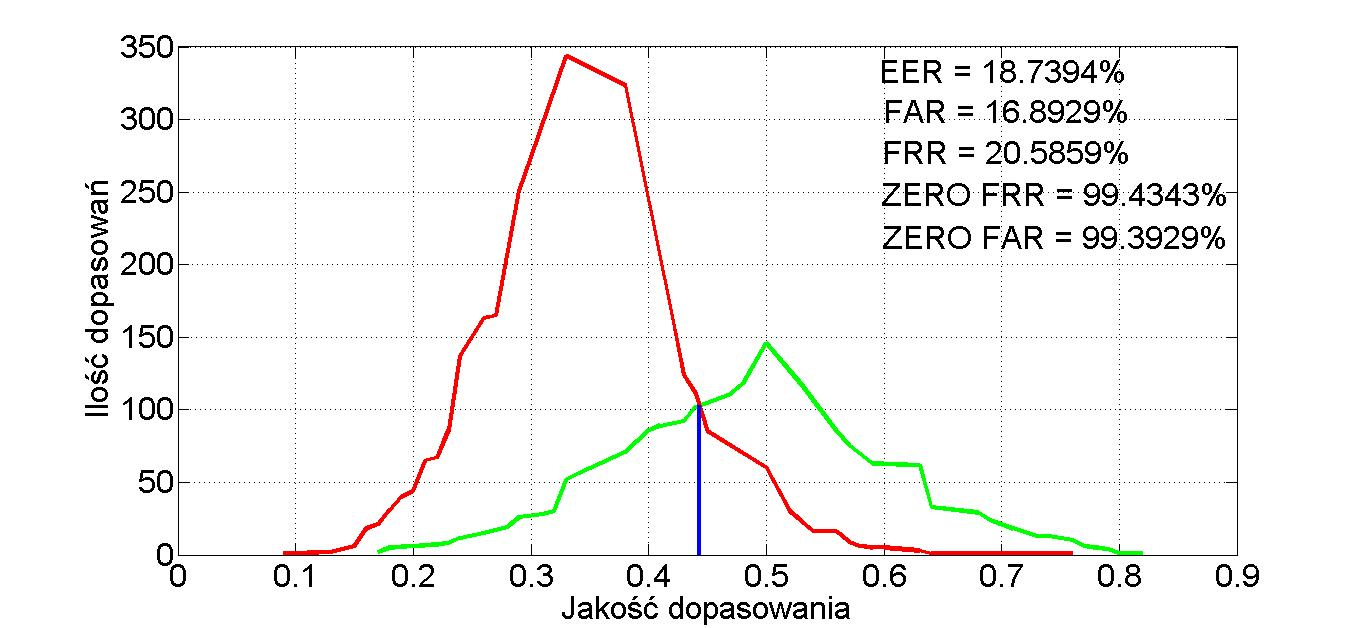
\includegraphics[angle=0,scale=0.35]{img/pattern_line_statistic_better_code.jpg}
		\caption{Ilość dopasowań w zależności od jakości dopasowania do odcisku wzorca (poprawiony algorytm)}
		\label{img:pattern_better_code}
    \end{center}
\end{figure} 

Wykresy \ref{img:pattern_better_code} oraz \ref{img:sample_better_code} prezentują wyniki poprawionego algorytmu. Wskaźnik EER poprawił się tylko nieznacznie z 17\%-21\% na 18\% - 19\%. FAR zmienił się z 11\% - 25\% na 13\% - 16\%. FRR z 17\% - 23\% na 21\% - 20\%. Jednak ogólna ocena mówi o niewielkiej zmianie przedstawionej modyfikacji algorytmu.

\begin{figure}[!htb]
    \begin{center}
		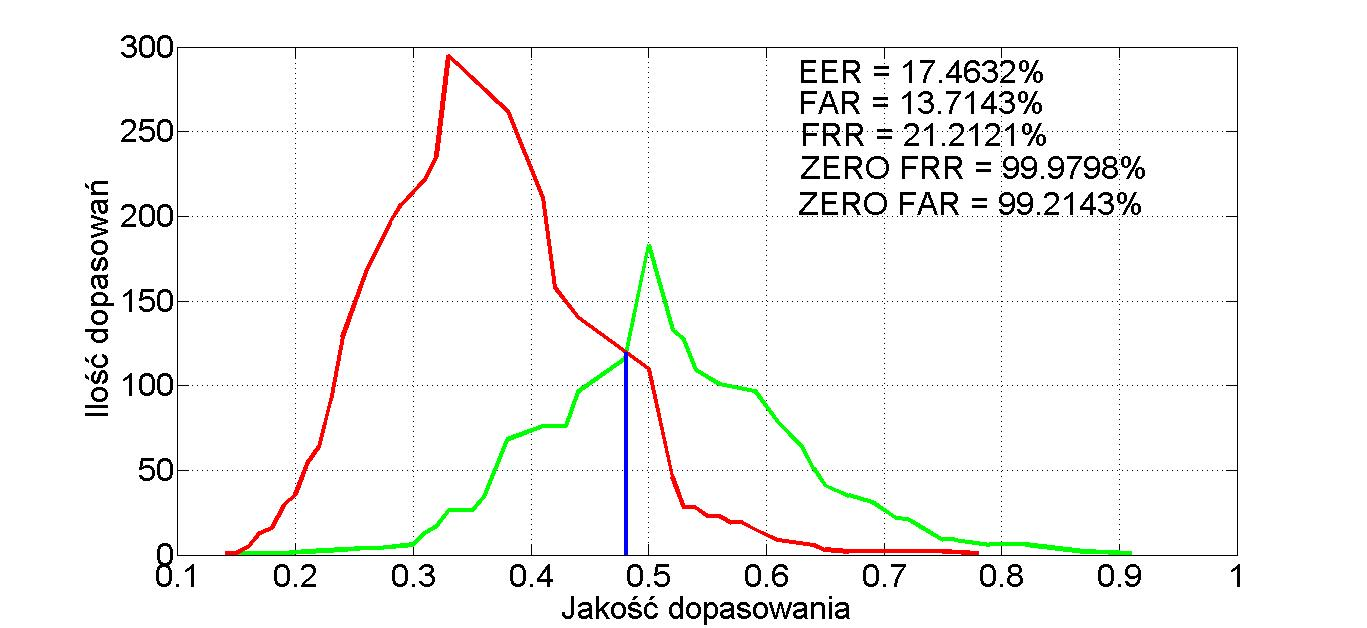
\includegraphics[angle=0,scale=0.35]{img/sample_line_statistic_better_code.jpg}
		\caption{Ilość dopasowań w zależności od jakości dopasowania do odcisku próbki (poprawiony algorytm)}
		\label{img:sample_better_code}
    \end{center}
\end{figure} 

Natomiast dal analizy różnicy symetrycznej wyniki nieco się poprawiły. EER spadł z 16\% na 13\%, FAR wzrósł z 12\% na 14\%, a FRR spadł z 17\% na 13\%. Wyniki przedstawione są na wykresie \ref{img:simetric_better_code}
\begin{figure}[!htb]
    \begin{center}
		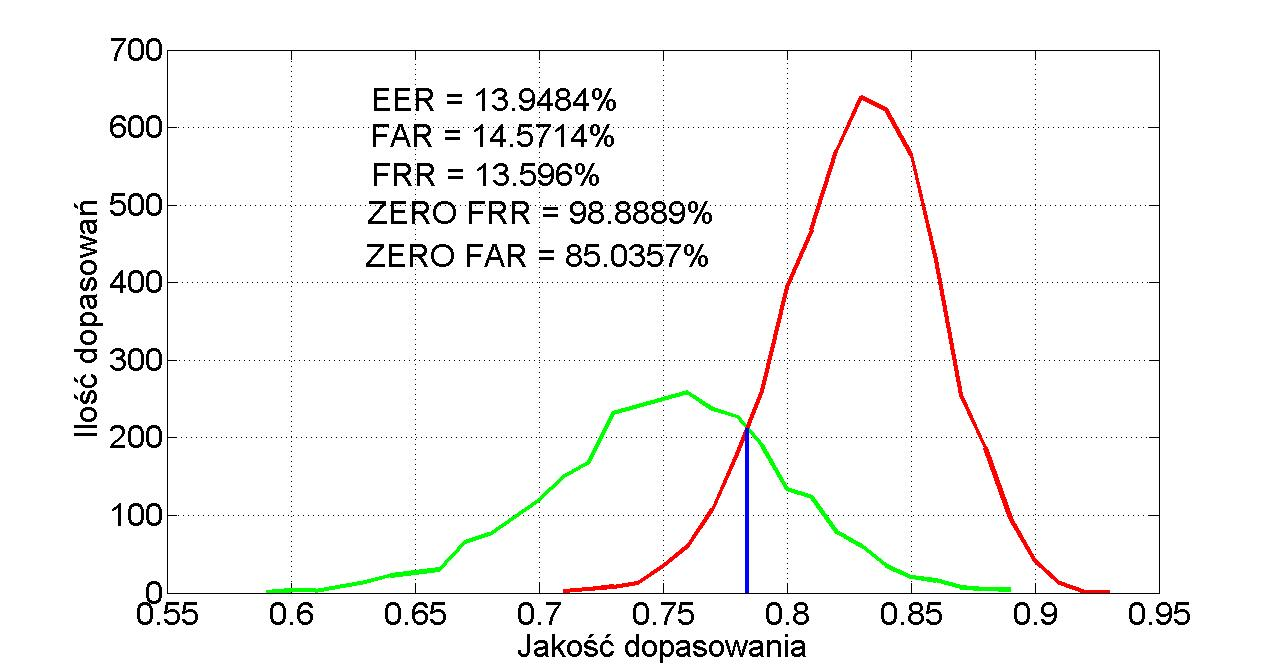
\includegraphics[angle=0,scale=0.4]{img/simetric_distance_better_code_line.jpg}
		\caption{Ilość niedopasowań w zależności od jakości niedopasowania do odcisków}
		\label{img:simetric_better_code}
    \end{center}
\end{figure} 

Tabele \ref{tab:3D_sum_21}, \ref{tab:3D_sum_22} i \ref{tab:3D_sum_23} przedstawiają wyniki metody 3D. Porównywania kodów również uzyskały podobne wyniki jak w niepoprawianej wersji algorytmu. Biorąc pod uwagę najlepszy wynik metod poprawiła się o ok 4 punkty procentowe. Globalnie metoda 3D tak jak i poprzednio wypadła znacznie gorzej niż analizowanie różnicy symetrycznej. Identycznie jak w poprzednich przypadkach przyczyną jest niemożliwość separowania zbiorów punktów porównań. 

\begin{table}[!htb]
    \begin{tabular}{p{3cm}|r||c|c|c|}
	\cline{2-5}
    & Wariant & \multicolumn{3}{|c|}{1:1 do 1:0 + 0:1}\\ \cline{2-5} 
    & Zbiór testujący & ERRORS  & FRR & FAR\\ \hline
	\multicolumn{2}{|l||}{Rodzaj jądra} &  \multicolumn{3}{|c|}{}\\
	\hline\hline
    \multicolumn{2}{|l||}{Liniowe} & 25.7359\% & 27.9635\% & 22.9755\%\\ \hline
    \multicolumn{2}{|l||}{Kwadratowe} & 26.1564\% & 31.1550\% & 19.9623\%\\ \hline
    \multicolumn{2}{|l||}{Wielomianowe st. 3} & 25.9882\% & 30.2432\% & 20.7156\%\\ \hline
    \multicolumn{2}{|l||}{Wielomianowe st. 7} & 29.5206\% & 31.6109\% & 26.9303\%\\ \hline
    \multicolumn{2}{|l||}{Wielomianowe st. 12} & 30.6981\% & 29.9392\% & 31.6384\%\\ \hline
    \multicolumn{2}{|l||}{Normalne(Gaussowskie)} & 26.0723\% & 33.2827\% & 17.1375\%\\ \hline
    \end{tabular}
	\caption{Wyniki testów poprawionego algorytmu kodowego metoda 3D porównywania kodów}
	\label{tab:3D_sum_21}
\end{table}

\begin{table}[!htb]
    \begin{tabular}{p{3cm}|r||c|c|c|}
	\cline{2-5}
    & Wariant & \multicolumn{3}{|c|}{1:1 do 1:0}\\ \cline{2-5} 
    & Zbiór testujący & ERRORS  & FRR & FAR\\ \hline
	\multicolumn{2}{|l||}{Rodzaj jądra} &  \multicolumn{3}{|c|}{}\\
	\hline\hline
    \multicolumn{2}{|l||}{Liniowe} & 31.2500\% & 19.0283\% & 48.3051\%\\ \hline
    \multicolumn{2}{|l||}{Kwadratowe} & 32.6651\% & 16.3968\% & 55.3672\%\\ \hline
    \multicolumn{2}{|l||}{Wielomianowe st. 3} & 31.8396\% & 17.4089\% & 51.9774\%\\ \hline
    \multicolumn{2}{|l||}{Wielomianowe st. 7} & 34.7877\% & 16.5992\% & 60.1695\%\\ \hline
    \multicolumn{2}{|l||}{Wielomianowe st. 12} & 35.6132\% & 15.9919\% & 62.9944\%\\ \hline
    \multicolumn{2}{|l||}{Normalne(Gaussowskie)} & 34.9057\% & 4.0486\% & 77.9661\%\\ \hline
    \end{tabular}
	\caption{Wyniki testów poprawionego algorytmu kodowego metoda 3D porównywania kodów}
	\label{tab:3D_sum_22}
\end{table}

\begin{table}[!htb]
    \begin{tabular}{p{3cm}|r||c|c|c|}
	\cline{2-5}
    & Wariant & \multicolumn{3}{|c|}{1:1 do 0:1}\\ \cline{2-5} 
    & Zbiór testujący & ERRORS  & FRR & FAR\\ \hline
	\multicolumn{2}{|l||}{Rodzaj jądra} &  \multicolumn{3}{|c|}{}\\
	\hline\hline
    \multicolumn{2}{|l||}{Liniowe} & 29.4652\% & 28.4872\% & 30.4979\%\\ \hline
    \multicolumn{2}{|l||}{Kwadratowe} & 30.5752\% & 34.5776\% & 26.3485\%\\ \hline
    \multicolumn{2}{|l||}{Wielomianowe st. 3} & 30.4743\% & 33.2024\% & 27.5934\%\\ \hline
    \multicolumn{2}{|l||}{Wielomianowe st. 7} & 30.4743\% & 32.6130\% & 28.2158\%\\ \hline
    \multicolumn{2}{|l||}{Wielomianowe st. 12} & 31.7861\% & 33.0059\% & 30.4979\%\\ \hline
    \multicolumn{2}{|l||}{Normalne(Gaussowskie)} & 29.9697\% & 34.9705\% & 24.6888\%\\ \hline
    \end{tabular}
	\caption{Wyniki testów poprawionego algorytmu kodowego metoda 3D porównywania kodów}
	\label{tab:3D_sum_23}
\end{table}


\vspace{5cm}\par
\section{Wnioski}
Oceniając zastosowane ulepszenie należy odnieść się do najlepszego uzyskanego wyniku, czyli analizy różnicy symetrycznej. Pomimo iż wskaźniki uległy poprawie nie należy uzyskanego wyniku uważać za satysfakcjonujący. 13\% wynik nie jest akceptowalny dla systemów biometrycznych. Dodatkowo próby uzyskania błędów zerowych kończą się podobnie jak w niepoprawianej wersji algorytmu. Dla takich progów błędy FAR i FRR wynoszą ponad 80\%. Świadczy to o wysokiej nieprzydatności zastosowanego rozwiązania. Pod sporym znakiem zapytania stoi również możliwość stosowania metod kodowania odcisku. Najważniejszym problemem jest niemożliwość spojrzenia na wszystkie minucje naraz. Oznacza to, że za każdym razem algorytm kodowania porównuje ze sobą dwa pojedyncze punkty i nie wie czy porównanie to ma jakikolwiek sens. Algorytmy obiektowe reprezentują minucje jako obiekty w programie, łatwe jest spojrzenie globalne na odcisk i wykluczanie dopasowań niemożliwych. Dla algorytmu kodującego porównanie kodu jest binarne i widzi on tylko pojedyncze elementy kodu.
\chapter{Implementacja algorytmu}

Implementacja algorytmu została wykonana w języku C++ z zastosowaniem standardowych bibliotek tego języka. Stworzony program to aplikacja konsolowa bez interfejsu użytkownika. Brak GUI motywowany jest koniecznością automatycznego wykonywania kodu na całej bazie danych obrazów. Dodatkowo aplikacja stanowi jedynie pomocnicze narzędzie do testowania wymyślonego algorytmu. Aplikacja składa się z trzech części modelu odcisku, czyli logicznego zapisu minucji dla każdego palca, silnika kodującego oraz silnika porównującego kody. Aplikacja jest jednowątkowa natomiast wszystkie funkcje napisane są w taki sposób aby w razie konieczności łatwo przerobić kod na wiele wątków. Aplikacja nie operuje na obrazach. Minucje są wydobywane za pomocą programu MINDTCT\footnote{Program MINDTCT jest częścią aplikacji NIST Fingerprint Image Software 2 wydaną przez Image Group of the National Institute of Standards and Technology}. Aplikacja jako wejście przyjmuje pliki .xyt zawierające położenia XY i kąta kolejnych minucji odcisku. Minucje oddzielone są znakiem enter. 
\newpage
\section {Diagram klas}
\begin{figure}[!hb]
    \begin{center}
		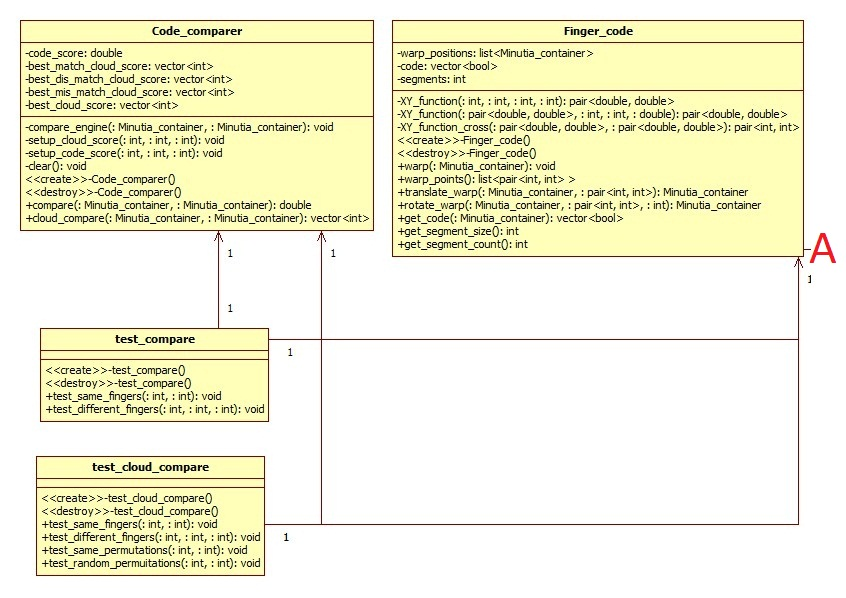
\includegraphics[angle=90,scale=.9]{img/UML_diagram_1.jpg}
		\caption{Diagram klas}
		\label{img:UML}
    \end{center}
\end{figure}
\newpage 
\begin{figure}[!hb]
    \begin{center}
		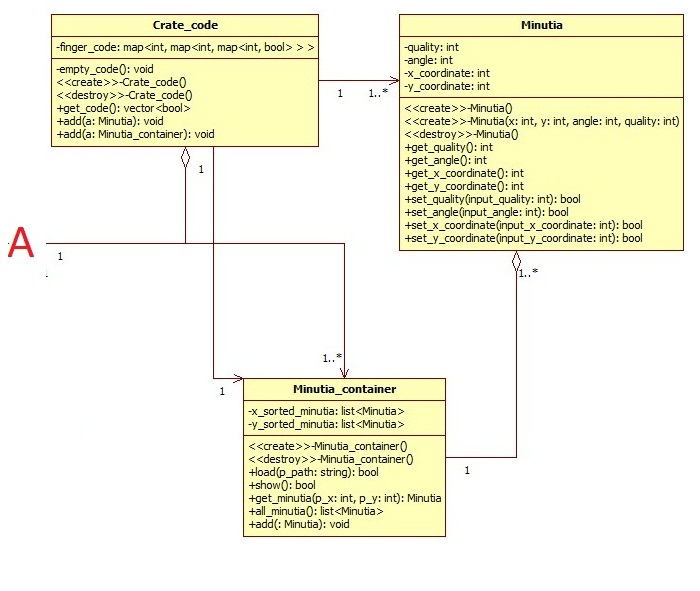
\includegraphics[angle=90,scale=.9]{img/UML_diagram_2.jpg}
		\caption{Diagram klas}
		\label{img:UML}
	\end{center}
\end{figure}

\section {Spis klas}
\begin{enumerate}
	\item Minutia
	\renewcommand*{\labelitemi}{\bullet}
	\begin{itemize}
		\item Klasa odzwierciedlająca fizyczny obiekt minucja. Stworzona do przechowywania podstawowych danych o minucji.
		\begin{itemize}
			\item kąt
			\item jakość
			\item położenie $x$
			\item położenie $y$
		\end{itemize}
		Klasa posiada podstawowe funkcje do zapisu i odczytu przechowywanych wartości.
	\end{itemize}
	\item Minutia\_container
	\renewcommand*{\labelitem}{\bullet}
	\begin{itemize}
		\item Klasa odzwierciedlająca fizyczny odcisk palca. Jest prostym kontenerem przechowującym Obiekty klasy $Minutia$. Jako kontener zastosowano $std::list$. Klasa przechowuje minucje posortowane po 
		współrzędnych, zarówno dla $x$ jak i $y$. 
		\begin{itemize}
			\item lista minucji posortowanych po współrzędnej $x$
			\item lista minucji posortowana po współrzędnej $y$
		\end{itemize}
		Klasa posiada funkcje do wczytywania listy minucji z pliku $.xyt$, Dodawania pojedyńczego obiektu typu $Minutia$, zwracania minucji po współrzędnych, zwracania wszystkich minucji, oraz mechanizm 
		wyświetlający wszystkie minucje na oknie konsoli(używane do debugowania). 
	\end{itemize}


	\item Crate\_code
	\renewcommand*{\labelitem}{\bullet}
	\begin{itemize}
		\item Klasa przechowująca pojedynczą zakodowaną transformacje na obrazie minucji. Jest fizyczną reprezentacją naiwnego kodu odcisku. 
		\begin{itemize}
			\item Naiwny kod
		\end{itemize}
		Klasa pozwala na dodawanie minucji oraz zbioru minucji do zakodowania. Posiada funkcje zwracającą utworzony kod, kod jest tworzony na bieżąco w momencie dodawania minucji.
	\end{itemize}
	\item Finger\_code
	\renewcommand*{\labelitem}{\bullet}
	\begin{itemize}
		\item Klasa przechowująca macierz kodów odcisku. Jest fizyczną reprezentacją całego kodu odcisku. Właściwie w funkcjach tej klasy zakodowany jest cały algorytm tworzący kod odcisku.
		\begin{itemize}
			\item Kod odcisku
			\item Liczba segmentów kodu
			\item Lista punktów transformacji obrazu(reprezentowana jako minucje do których należy przesunąć obraz)
		\end{itemize}
		Klasa posiada funkcje do zwrócenia kodu odcisku, pobrania rozmiaru segmentu kodu, liczby segmentów, oraz funkcje dokonujące transformacji obrazu.
	\end{itemize}
	\item Code\_comparer
	\renewcommand*{\labelitem}{\bullet}
	\begin{itemize}
		\item Klasa obliczająca stopień dopasowania odcisków, jest fizyczną reprezentacja funkcji porównującej kody. W zależności od wywoływanej funkcji zwraca odpowiedni współczynnik dopasowania. Działa w 
		dwóch trybach zwracając liczbę minucji dopasowanych i niedopasowanych, lub oblicza współczynnik dopasowania na podstawie podanych wag. 
		\begin{itemize}
			\item najlepszy współczynnik dopasowania
			\item liczby dopasowań, niedopasowań, maksymalizujące liczbę porównań 1:1
			\item liczby dopasowań, niedopasowań, minimalizujące liczbę porównań 1:0
			\item liczby dopasowań, niedopasowań, minimalizujące liczbę porównań 0:1
			\item najlepszą liczbę dopasowań, niedopasowań, arbitralnie wybrany wskaźnik maksymalizujący liczbę porównań 1:1
		\end{itemize}
		Klasa posiada silnik porównujący podane kody, oraz metody obliczające dopasowanie dla dwóch trybów działania.
	\end{itemize}
	\item Test\_compare
	\renewcommand*{\labelitem}{\bullet}
	\begin{itemize}
		\item Klasa do testowania mechanizmu porównywanie poprzez obliczanie współczynnika porównań.
	\end{itemize}
	\item Test\_cloud\_compare
	\renewcommand*{\labelitem}{\bullet}
	\begin{itemize}
		\item Klasa do testowania mechanizmu porównywanie poprzez obliczanie liczby dopasowań niedopasowań.
	\end{itemize}
	\item Config.h
	\renewcommand*{\labelitem}{\bullet}
	\begin{itemize}
		\item Plik nagłówkowy zawierający elementy konfiguracji programu.
	\end{itemize}
\end{enumerate}



\begin{lstlisting}[language=C++,style=outcode,caption=Przykładowa konfiguracja]
/*
 * Config.h
 *
 *  Created on: 2011-05-07
 *      Author: czareq
 */

#ifndef Config_H_
#define Config_H_

#include <limits.h>

#define ERROR INT_MAX
#define MIN_SCORE INT_MIN
const double PI = 3.14159265358979323851280895940;

/*
 * code parameters
 */
const int X_CODE_RES = 300;
const int Y_CODE_RES = 300;
const int ANGLE_RES = 300;
const int CODE_SEP = 25; 
const int CODE_ANGLE_SEP = 30;

/*
 * warper parameters
 */
const double COVER_STEP = 0.5; 
const int X_STEP = (int) (COVER_STEP * CODE_SEP);
const int Y_STEP = (int) (COVER_STEP * CODE_SEP);
const int ANGLE_STEP = 15;
const int ANGLE_STEP_RANGE = 45;

/*
 * comparer parameters
 */
const int MATCH_POINT = 500;
const int DIS_MATCH_POINT = 500;
const int MIS_MATCH_SCORE = 100;
#endif /* Config_H_ */
\end{lstlisting}
\section {Przebieg procesu weryfikacji}

\begin{enumerate}
	\item Wyodrębnienie listy minucji minucji
	\renewcommand*{\labelitem}{\bullet}
	\begin{itemize}
		\item MINDTCT ekstrakcaj minucji wzorca i próbki
		\item Zapis do pliku $.xyt$
	\end{itemize}
	\item Tworzenie modeli
	\renewcommand*{\labelitem}{\bullet}
	\begin{itemize}
		\item Wczytanie plików $.xyt$
		\item Utworzenie obiektu $Minutia\_container$ dla wzorca i dla próbki oraz zapisanie w nich obiektów $Minutia$
	\end{itemize}
	\item Tworzenie kodów
	\renewcommand*{\labelitem}{\bullet}
	\begin{itemize}
		\item Utworzenie obiektu $Crate\_code$ dla wzorca
		\item Utworzenie obiektu $Finger\_code$ dla próbki
		\item Zakodowanie próbki
		\begin{itemize}
			\item Utworzenie listy wszystkich translacji
			\item Utworzenie listy obrotów dla każdej translacji
			\item Utworzenie obiektu $Crate\_code$ dla każdej transformacji
			\item Dodanie obiektów $Crate\_code$ do obiektu $Finger_code$
		\end{itemize}
	\end{itemize}
	\item Weryfikacja
	\renewcommand*{\labelitem}{\bullet}
	\begin{itemize}
		\item Utworzenie obiektu $Code_compare$
		\item Pobranie kodu wzorca
		\item Pobranie kodu próbki
		\item Podział kodu próbki na segmenty
		\item Porównanie kodu wzorca z każdym z kodów segmentu
	\end{itemize}
	\item Zwrócenie i zapisanie wyniku
	\renewcommand*{\labelitem}{\bullet}
	\begin{itemize}
		\item Odczytanie najlepszego wyniku porównania
		\item Zapis do pliku
	\end{itemize}
\end{enumerate}
\chapter{Weryfikacja obiektowo-kodowa}

Ocenę metod weryfikacji odcisków należy wystawić przede wszystkim na podstawie ilości błędów popełnianych przez obie metody. W takim przypadku metody obiektowe zostawiają daleko w tyle opisywaną metodę kodową. Błędy EER w granicach 16\% -20\% świadczą o dużej zawodności metody. W książce  \emph{Handbook of fingerprint recognition} \cite{finger_book} prezentowana jest tabela prezentująca błędy EER dla znanych algorytmów porównywania odcisków. W czołówce znajdują się algorytmy o EER poniżej 1\%, a najlepszy przedstawiany algorytm (PA15) ma skuteczność na poziomie 0.19\%. Tabele zamykają algorytmy o skuteczności 12\%- 16\%, 23\% i 50\%. Oznacza to, że moje rozwiązanie mogłoby być porównywane z niektórymi najsłabszymi algorytmami przedstawianymi w książce. Najgorsze komercyjne rozwiązanie ma skuteczność 12.09\% co oznacza, że mój algorytm jest niewiele gorszy. Dodatkowo w przypadku prób zapewnienia zerowych błędów fałszywej akceptacji lub fałszywego odrzucenia algorytm staje się kompletnie bezużyteczny. Jednak metoda niekoniecznie musi zostać porzucona warto zauważyć, że algorytm kodujący nie korzysta z żadnych zaawansowanych metod. Jest to tylko wyłącznie proste kodowanie poprzez podzielenie przestrzeni na mniejsze fragmenty i stwierdzanie czy minucja znajduje się w niej czy też nie. Ciężko wyciągać wnioski bez przeprowadzenia eksperymentu, ale gdyby zamiast określać miejsca w którym znajduje się minucja określać gdzie znajduje się z pewnym prawdopodobieństwem to metoda kodowa mogłaby być skuteczniejsza. Jednak takie podejście nie mówi wprost o ilości dopasowanych minucji. I prawdopodobnie również byłoby nieskuteczne dowodzi tego test przeprowadzony w poprzednim rozdziale. Porównywano tam nie tylko bezpośrednio odpowiadające kratki kodu ale też i sąsiednie. W obecnym podejściu algorytm podejmuje binarne decyzje co do dopasowania minucji. Wersja z kodowaniem prawdopodobieństwa położenia minucji w danym obszarze stwierdza dopasowanie minucji wraz z prawdopodobieństwem. Reasumując niełatwe jest wtedy stwierdzenie ile minucji dopasowano a ile nie. Podejście takie utrudniałoby badanie podobieństwa i niepodobieństwa obrazów na podstawie liczby dopasowanych i niedopasowanych minucji, a właśnie takie założenie przyjmuje ta praca. Innym sposobem poprawy jest znalezienie sposobu na kompensacje nieliniowych odkształceń opuszka palca w procesie pobierania odcisku. W aktualnym rozwiązaniu stosowane są przekształcenia(obroty i przesunięcia) dla całego obrazu. Nie stosowane są lokalne transformacje obrazu. Nie jasny jest też sposób realizacji takich przekształceń. Możliwym problemem wprowadzenia tego pomysłu jest nieskończony zbiór przekształceń jaki można wykonać na obrazie. Mówiąc prościej i tak należałoby arbitralnie wybrać jakąś grupę przekształceń bez pewności, że wśród nich znajduje się przekształcenie kompensujące zniekształcenia w obrazie. Tak naprawdę bardzo trudno jest znaleźć dobre wyjście z tego problemu, bo nie wiadomo co jest poszukiwane. Dobrym kierunkiem rozwoju metody jest, wspomniane powyżej, kompletne odejście od liczby dopasowanych minucji. Algorytm stwierdzi jedynie ważone prawdopodobieństwo dopasowania obrazu. Rozwiązanie takie różni się od obecnego tym, że zniekształcenia obrazu są kompensowane nie tylko przez rozmiar kratki kodu ale również przez przynależność do sąsiednich kratek. Jest to jednak temat na kolejne badania.
\section [Ocena i porównanie metod][Ocena i porównanie metod]{Ocena i porównanie metod}
Kolejnym etapem pracy było stworzenie mechanizmu porównywania kodów. Rozważano kilka sposobów porównań.
\renewcommand*{\labelitemi}{\bullet}
\begin{itemize}
	\item porównywanie naiwnego kodu
	\item porównywanie macierzy kodów(transformacje na obrazie próbki)
	\begin{itemize}
		\item porównywanie podobieństwa
		\item porównywanie niepodobieństwa
		\item porównywanie podobieństwa i niepodobieństwa jednocześnie(3D)
	\end{itemize}
\end{itemize}
Dla algorytmu kodującego najskuteczniejsze okazało się porównywanie niepodobieństwa i transformacje obrazu próbki. Dla liczby minucji dopasowanych i niedopasowanych pozyskiwanych od SDK $Neurotechnology$ najskuteczniejszą metodą okazała się metoda 3D porównywania kodów. Skuteczność takiego porównania daje wynik w granicach 0.5\% błędnych decyzji. Wynik ten śmiało mógłby rywalizować z przedstawianym algorytmami w książce $Handbook of fingerprint recognition$\cite{finger_book}. Niestety nie jest to moje autorskie rozwiązanie a jedynie wykorzystanie komercyjnego SDK w połączeniu z moją metodą. Wynik jednak jest bardzo dobry i taki system mógłby być działającym powszechnie systemem biometrycznym. Konieczne jest jedynie nauczenie klasyfikatora SVM odpowiedniej funkcji separującej. W opisywanej pracy funkcje zostały otrzymane na niezbyt dużych bazach danych. Zwiększenie zbioru uczącego przyczyni się do większego generalizowania zachowania rozkładu ilości punktów dopasowanych i niedopasowanych minucji. Metoda ta nie jest uniwersalna, oznacza to ze proces uczenia klasyfikatora powinien być dostosowywany do oprogramowania, które oblicza liczby dopasowanych i niedopasowanych cech. Jak każda metoda tak i ta posiada wady. Ten sposób klasyfikacji nie daje oczekiwanych rezultatów gdy zbiór punktów dopasowania i zbiór punktów niedopasowania nie jest rozłączny. W przypadku przedstawianego algorytmu kodującego metoda te prowadzi wręcz do pogorszenia wyników. 




\appendix

% tutaj załączniki

%\chapter*{Bibliografia}
\nocite{*}
\bibliographystyle{plplain}
%\bibliographystylebk{plplain}
%\bibliographystylest{plplain}
%\bibliographystyledoc{plplain}
% \bibliographystyleweb{plplain}
%\bibliographybk{BIB/books}
%\bibliographyst{BIB/books}
%\bibliographydoc{BIB/books}
% \bibliographyweb{BIB/books}

% \bibliography{bib/verificard,bib/jml,bib/daikon}
\bibliography{bib/books}

\end{document}

% ex: set tabstop=4 shiftwidth=4 softtabstop=4 noexpandtab fileformat=unix filetype=tex spelllang=pl,en spell:

